\documentclass[twoside,11pt]{starlink}
\usepackage{graphicx}
\usepackage{float}
\usepackage[labelformat=empty]{subfig}
\usepackage[font=footnotesize]{caption}

\stardocauthors     {D.S. Berry }
\stardocdate        {6th July 2016}
\stardoctitle       {POL-2 Data Reduction}
\stardocversion     {V1.0}
\stardocabstract    {POL-2 data reduction: a description and analysis of the methods used}

\begin{document}
\scfrontmatter
\section{Overview}

Reduction and analysis of raw POL-2 data involves the following steps:

\begin{enumerate}
\item Creation of  Q and U time-streams from the raw analysed intensity time-stream data.
\item Creation of Q and U maps from the Q and U time-stream data
\item Creation of vector catalogues from the Q and U maps.
\item Display and analysis of the final vector catalogues.
\end{enumerate}

Later sections of this document describe the above steps. They adopt the
nomenclature and conventions of the Starlink \xref{POLPACK}{sun223}{}
package. In particularly, see the section of SUN/223 on \xref{Single Beam
Polarimetry}{sun223}{singlebeampolarimetry}. In the context of that
document POL-2 corresponds to a ``type 3'' polarimeter, containing a
fixed analyser and a spinning half-wave plate. It is assumed that POL-2
has an \emph{analyser efficiency} of unity. The \emph{analyser
transmission} is incorporated into the results at a later point (the
calibration stage) via the Flux Conversion Factor - FCF. In this section
we therefore assume a value of unity for the analyser transmission.

The fixed analyser in POL-2 consists of a set of wires that are
accurately parallel to the focal plane Y axis, meaning that it passes
signal that is polarised parallel to the focal plane X axis. This means
that the $ANGROT$ value, as defined in the above POLPACK references,
is zero.

\section{The raw data}
Raw POL-2 data files contain a time-stream for each bolometer, sampled at
a nominal frequency of 175 Hz, containing the analysed intensity value at
each sample. The values are in arbitrary integer units determined by the
hardware analogue to digital converters, and need converting to floating
point power values in units pW before being used (see the section on
``flat-fielding'' below). Each bolometer time-stream is a periodic
function of time containing several different harmonics of the half-wave
plate rotation (see Figs.~\ref{fig:rawdata} and ~\ref{fig:rawfft}). The
half-wave plate spins at a frequency of 2 Hz, and so information about
the astronomical Q and U signals are given by the amplitude and phase of
the 8 Hz component of each time-stream (see the POLPACK references
above). However, other harmonics are also present - the 4 Hz signal is
very strong, with additional significant signal present at 2 Hz and 16
Hz\footnote{The source of these other harmonics is thought to be standing
waves caused by reflections between the half-wave plate and the fixed
analyser.}. These periodic signals are superimposed on a slowly varying
background value that represents a combination of total intensity from
the sky and astronomical source, plus any base line drifts caused by the
detectors and electronics.

\begin{figure}
\includegraphics[width=\columnwidth]{rawdata}
\caption{A typical section of raw POL2 data from bolometer (20,20) an
observation of Orion A (20160125 observation 31). The 10 second section on
the left illustrates the slowly varying background, whilst the 1 second
section on the right shows the strong 4 Hz signal and weaker 8 Hz signal.
The numbers on the vertical axes show raw (\emph{i.e.} unflatfielded) values in
ADU units.}
\label{fig:rawdata}
\end{figure}

\begin{figure}
\includegraphics[width=\columnwidth]{rawfft}
\caption{The power spectral density of the same data (after
flat-fielding) shown in Fig.~\ref{fig:rawdata}. The left hand plot has a
linear vertical axis and shows the strong 4 Hz and 8Hz signal. The right
hand plot has a logarithmic vertical axis and shows that several other
harmonics (multiples of 2 Hz) are present at a lower level. The majority
of the 8 Hz signal is produced by instrumental polarisation of the sky
background.}
\label{fig:rawfft}
\end{figure}


\subsection{The angular zero-point of the half-wave plate}
\label{sec:rawcal}
The half-wave plate (HWP) spins at 2 Hz during a POL-2 observation, and
its orientation at each sample is recorded in the $POLANG$ array within
the JCMTSTATE extension of each raw data file. The $POLANG$ values give
the angle between the focal plane X axis and some arbitrary fixed line on
the HWP, measured positive in the sense of rotation from focal plane Y to
focal plane X. The mathematical theory presented in the POLPACK
references above refer to the angle, $WPLATE$, from the fixed analyser
(which is parallel to the focal plane X axis in the case of POL-2) to the
fast axis of the HWP. The $POLANG$ and $WPLATE$ values are connected as
follows:

\[ WPLATE = PAOFF - POLANG \]

where $PAOFF$ is a constant fixed offset that gives the angle between the
HWP fast axis and the line corresponding to zero $POLANG$\footnote{The
minus sign is there because POLPACK defines positive angles from X to Y,
which is opposite to the sense in which $POLANG$ is defined.}. To
determine the value of $PAOFF$, observations were taken with the dome
closed and the POL-2 calibrator in-beam. Closing the dome ensure that the
observed total intensity is constant throughout the observation.
Inserting the calibrator into the beam causes the measured intensity to
be virtually 100\% polarised with an accurately known direction - parallel
to the focal plane X axis\footnote{The resulting analysed intensity is
so strong that the usual flat-fielding algorithm fails, flagging all
bolometers as bad. Therefore analysis of this data is done without
flat-fielding. This should not be a problem since we are only interested
in ratios of Q and U here.}.

Below is equation (1) from SUN/223
\xref{Single Beam Polarimetry}{sun223}{singlebeampolarimetry} (with the
HWP transmission and efficiency set to 1.0):

\[ I_{rec} = \frac{1}{2}( I + Q.\cos 2\phi + U.\sin 2\phi ) \]

where $I_{rec}$ is the recorded analysed intensity, $I$, $Q$ and $U$ are
the Stokes parameters describing the polarisation with respect to a
reference direction parallel to the fixed analyser (\emph{i.e.} the focal
plane X axis), and

\[ \phi = 2.WPLATE \]

Using $PAOFF$ and $POLANG$ in place of $\phi$, this becomes:

\[ I_{rec} = \frac{1}{2}( I + Q.\cos(4.PAOFF - 4.POLANG) + U.\sin(4.PAOFF - 4.POLANG) ) \]

which can be re-arranged to:

\[ I_{rec} = \frac{1}{2}( I + Q'.\cos 2\phi' + U'.\sin 2\phi' ) \]

where

\[ \phi' = -4.POLANG \]
\[ Q' = Q.\cos( 4.PAOFF ) + U.\sin( 4.PAOFF )\]
\[ U' = -Q.\sin( 4.PAOFF ) + U.\cos( 4.PAOFF )\]

In other words, $\phi'$, $Q'$ and $U'$ are the values of $\phi$, $Q$
and $U$ that would be measured if a non-zero $PAOFF$ was simply ignored
(\emph{i.e.} assumed to be zero).

If the angle from the fixed analyser to the actual polarisation vector is
$\theta$, then:

\[ Q = I_p.\cos 2\theta \]
\[ U = I_p.\sin 2\theta \]

Substituting for $Q$ and $U$ in the above expressions for $Q'$ and $U'$
gives:

\[ Q' = I_p.\cos 2\theta.\cos( 4.PAOFF ) + I_p.\sin 2\theta.\sin( 4.PAOFF )\]
\[ U' = -I_p.\cos 2\theta.\sin( 4.PAOFF ) + I_p.\sin 2\theta.\cos( 4.PAOFF )\]

which can be re-arranged to:

\[ Q' = I_p.\cos 2\theta' \]
\[ U' = I_p.\sin 2\theta' \]

where

\[ \theta' = \theta - 2.PAOFF \]

That is, $\theta'$ is the polarisation angle that would be measured if
$PAOFF$ was simply ignored (\emph{i.e.} assumed to be zero).

In the case of POL-2 observation of the dome with the calibrator in-beam,
we know that the true angle, $\theta$, is zero (\emph{i.e.} the calibrator
produces polarisation that is parallel to the focal plane X axis), and so:

\[ PAOFF = -\frac{1}{2}.\theta' \]

To determine $\theta'$ we generate $Q'$ and $U'$ values from the POL-2
observations using the {\texttt smurf:calcqu} command, setting the $PAOFF$
configuration parameter to zero. We then calculate a $\theta'$ value for
each sample using:

\[ \theta' = \frac{1}{2}.atan2( U' ,Q' ) \]

Fig.\ref{fig:paoff} shows histograms of measured angles for two such
observations (20151002 observation 115 and 20151003 observation 1). We
adopt 52.7$^\circ$ as a representative angle for all
sub-arrays\footnote{Although there seem to be systematic differences
between sub-arrays and spatial structures which are as yet unexplained.}.
These angles are measured from focal plane Y towards negative focal plane
X, so we need to change it to the convention used by $\theta'$ (from
focal plane X towards focal plane Y):

\[ \theta' = -( 90 - 52.7 ) = -37.3^\circ \]

So finally:

\[ PAOFF = -\frac{1}{2}.\theta' = 18.65^\circ \]

\begin{figure}
\includegraphics[width=\columnwidth]{paoff}
\caption{The measured polarisation angles assuming zero
$PAOFF$ obtained from two POL-2 observations of the dome with the calibrator
in-beam. Colour indicates sub-array - black:S8A, red:S8B, blue:S8C,
green:S8D.}
\label{fig:paoff}
\end{figure}

As a test, we re-run \texttt{smurf:calcqu} supplying 18.65$^\circ$ as the value
for the PAOFF configuration parameter. The resulting histograms of angle
values in Fig.\ref{fig:paoff2} show that setting $PAOFF = 18.65^\circ$
does indeed result in the polarisation produces by the calibrator being
reported as parallel to the focal plane X axis (\emph{i.e.} $90^\circ$
from the focal plane Y axis).

\begin{figure}
\includegraphics[width=\columnwidth]{paoff2}
\caption{The measured polarisation angles assuming $PAOFF=18.65^\circ$
- see Fig.\ref{fig:paoff}.}
\label{fig:paoff2}
\end{figure}

\subsection{The analysed intensity waveform}
\label{sec:wave}
The time-stream from each bolometer is a periodic function of time as
described above, containing several harmonics of the HWP rotation. The
fourth harmonic (8 Hz) carries the astronomical signal. For a perfect
HWP, this astronomical signal should be given by:

\[ I_{rec} = \frac{1}{2}( I + Q.\cos 2\phi + U.\sin 2\phi ) \]

In other words, the astronomical signal should be a sine wave of
frequency 8 Hz with a zero-point offset given by $I$. For observations
that include the calibrator (described in the previous section), the 8 Hz
signal is very strong and dominates the 2 and 4 Hz signal.
Fig.~\ref{fig:calib-wave} shows the mean waveform seen in such an
observation (observation 115 on 20151002). This plot was formed by
first flat-fielding and cleaning the data (which includes removing a
linear background from each bolometer), then finding the mean value
at each time slice and then binning these mean values according to
the corrected $POLANG$ value\footnote{The correction consists of
subtracting off the zero-point offset of $18.65^\circ$ described
in the previous section.}. It can be seen that the waveform is far
from sinusoidal, with flat peaks and sharp troughs.

\begin{figure}
\includegraphics[width=\columnwidth]{calib-wave}
\caption{The mean waveform in the analysed intensity data for a
calibrator observation.}
\label{fig:calib-wave}
\end{figure}

This non-sinusoidal waveform could potentially be caused by imperfections
in the HWP, but could also be caused by the very strong polarised
intensity generated by the calibrator pushing the hardware into a
non-linear regime. The flat-fielding is a particular problem. The normal
flat-fielding method based on using a fast-flat taken at the start of the
observation could not be used in this case as the strong signal resulted in all
bolometers being rejected. Instead, each sub-scan was flatfielded
individually using \texttt{smurf:flatfield} so that the flat-field
parameters stored internally within each file were used. It is possible
that the flat-fielding is not correctly taking account of non-linearities
in the detectors at these very high signal levels.

To check this hypothesis, a similar analysis was done for a genuine
on-sky observation of a field with no significant astronomical polarised
intensity (observation 36 on 20160419 - CB 68). Fig.~\ref{fig:cb68-wave2}
shows the mean waveform as a function of HWP position. In this case,
the 8 Hz signal (caused by instrumental polarisation of the unpolarised
sky signal) is much weaker than for the above calibrator observation,
bringing it down to the level of the 2 and 4 Hz signal. This makes the
waveform harder to interpret. However, the \texttt{calcqu} command can
be modified to remove 2 and 4 Hz signal and so simplify the waveform.
To calculate Q and U, \texttt{calcqu} performs a least squares fit to
every half second of data from each bolometer. The fit includes 2, 4, 8
and 16 Hz sine and cosine waves, and a linear background. The modified
\texttt{calcqu} removes the linear background and the evaluated 2 and
4 Hz signal from the input data to create the output data from which
the mean waveform shown in Fig.~\ref{fig:cb68-wave} (the red dots)
is determined (the blue line shows the fitted 8 Hz sine wave). This
waveform looks much more sinusoidal than that shown in
Fig.~\ref{fig:calib-wave}, suggesting that it is indeed the strength
of the polarised intensity created by the calibrator that is causing
the bulk of the problems in Fig.~\ref{fig:calib-wave}.

\begin{figure}
\includegraphics[width=\columnwidth]{cb68-wave2}
\caption{The mean waveform in the analysed intensity data for an
on-sky observation of CB 68.}
\label{fig:cb68-wave2}
\end{figure}

\begin{figure}
\includegraphics[width=\columnwidth]{cb68-wave}
\caption{The mean analysed intensity waveform for CB 68, after removal of
2 and 4 Hz signal. The blue line indicates the fitted 8 Hz sine wave.}
\label{fig:cb68-wave}
\end{figure}

Fig.~\ref{fig:cb68-scat} show a scatter plot of the waveform values after
removal of 2 and 4 Hz signal, against the fitted 8 Hz waveform values
(that is, a scatter plot of the corresponding red and blue values from
Fig.~\ref{fig:calib-wave}). This scatter plot shows a distinct curve,
implying some non-linearity remains even at this lower level of
polarised intensity. This is the sort of effect you might see if the
transmission of the HWP was not constant but varied with the angle
between the incoming plane of polarisation and the HWP fast axis.

The 16 Hz component present in the analysed intensity time-streams could
be another indication of the same non-linearity, and could result in the
same sort of curve seen in Fig.~\ref{fig:cb68-scat}.

Further work is needed to determine if this curve is due to variable
transmission in the HWP or some similar issue with the HWP, and whether
it can be quantified and corrected.

\begin{figure}
\includegraphics[width=\columnwidth]{cb68-scat}
\caption{The fitted 8 Hz signal plotted against the actual waveform values for
CB 68 (after removal of 2 and 4 Hz signals).}
\label{fig:cb68-scat}
\end{figure}





\section{Creation of  Q and U time-streams}

This section describes the process of converting raw analysed intensity
time-stream data sampled at 175 Hz, into pairs of time-streams holding  Q
and U values sampled at 2 Hz (\emph{i.e.} one Q/U sample is created for
each rotation of the half-wave plate), in units of $pW$. The \texttt{smurf:calcqu}
command does this conversion. The Q time-streams and U time-streams
are stored in separate output files.

\subsection{Cleaning}

The details of the cleaning applied to the raw analysed-intensity data prior
to calculating Q and U values can be controlled via the CONFIG parameter
of the \texttt{smurf:calcqu} command. By default, it includes the
following operations in the stated order:

\begin{enumerate}
\item Apply flat-field and convert to units of $pW$
\item Identify and fix steps in the DC offset of each bolometer time-stream
\item Identify and remove transient spikes in each  bolometer time-stream
\item Remove a constant offset from each bolometer time-stream
\item Correct POL-2 triggering issue.
\end{enumerate}

\subsubsection{Flat-fielding}
Raw POL-2 (\emph{i.e.} analysed  intensity) data is flat-fielded and
scaled into units of $pW$ using fast flatfield ``ramps'' taken at the start
and end of each observation. The method used is exactly the same as that used
for SCUBA-2 scan maps.

\subsubsection{Fix DC steps}
\label{sec:steps}
DC steps in the raw analysed intensity look very much like steps seen in
non-POL-2 data. For instance, Fig.~\ref{fig:steps1} shows the analysed
intensity time-stream for typical bolometer, including an obvious DC
step. The top panel shows the analysed intensity time-stream after the
step has been fixed\footnote{A step is fixed by adding a constant value
onto either side of the step such that the overall mean value remains
unchanged and the height of the step is minimised.}. It is clear that the
step does not simply cause a change in the DC offset of the bolometer, but also
causes a change in the \emph{gain} of the bolometer, as indicated by the
sudden change in the amplitude of the oscillations on either side of the
step\footnote{This change in gain causes a sudden step in the polarised
intensity, which is fixed when cleaning the Q/U time-streams in
\texttt{makemap}.}. Fig.~\ref{fig:steps2} shows the resulting Q and U time-streams over
the whole length of the observation. Clearly the step is introducing some
sort of noise into the time-stream that makes the data that follows the
step effectively unusable. Fig.~\ref{fig:steps3} shows data for a few
rotations of the half-wave plate. The effect of the increased noise after
the step can be seen. The \texttt{calcqu} command stores a variance
for each output Q and U value, which is the square of the RMS residual
between the analysed intensity data and the least squares fit.
Fig.~\ref{fig:steps4} shows the square root of these variances,
showing that the noise nearly doubles following the step. Currently, no
attempt is made to identify and remove these noisy sections of data.
However, they will be down-weighted in the map due to their higher
variances.

It is possible that this instability following a step may be related to
the flattening of the raw data streams described in
\url{https://www.eao.hawaii.edu/pol2/Commissioning%20Reports}~.
Maybe the step moves the data values into a region where the flat-field
ramp is unreliable.

Fixing steps in the analysed intensity time-streams has a relatively
small effect on the final maps. This is because the measured Q/U values
are independent of shifts in the baseline. The main reason for fixing
steps in normal SCUBA-2 scan maps is to avoid ringing in the high-pass
filter. However, no such filtering is used when creating Q/U values and
so ringing is not a problem.

\begin{figure}
\includegraphics[width=\columnwidth]{steps1}
\caption{A typical step in the analysed intensity time-stream of S8A bolometer
(26,6) in observation 31 from 20160125 (Orion A). The lower plot shows
the whole 50 minute observation, the middle plot shows a 30 second
section around the step, and the top plot shows the time-stream after the
step has been fixed.}
\label{fig:steps1}
\end{figure}

\begin{figure}
\includegraphics[width=\columnwidth]{steps2}
\caption{The entire Q and U time-streams derived from the step-fixed data
shown in Fig.~\ref{fig:steps1}. The step seems to cause Data following
the step seems to have extremely bad Q and U values. Note, the time values
on the horizontal
axis are wrong in these plots - there is currently a bug in \texttt{calcqu}
that invalidates the time WCS information in the output time-streams.
However the final Q and U maps are unaffected by this bug since
\texttt{makemap} does not use the WCS information.}
\label{fig:steps2}
\end{figure}

\begin{figure}
\includegraphics[width=\columnwidth]{steps3}
\caption{Small sections of the analysed intensity time-stream before
(lower plot) and after (upper plot) the step. The increased noise is
visible. }
\label{fig:steps3}
\end{figure}

\begin{figure}
\includegraphics[width=\columnwidth]{steps4}
\caption{The noise in the Q and U values shown in Fig.~\ref{fig:steps2}.
The whole time-stream is shown.}
\label{fig:steps4}
\end{figure}

\subsubsection{Remove transient spikes}
Each bolometer is processed independently. At each time slice, the
median value of the bolometer is found within a box of 50 samples
(\emph{i.e.} about 0.3 seconds) centred on the time slice. If the
difference between the time slice value and the median value is greater
than 5 times the local noise level, the time slice is flagged as
a spike and is subsequently ignored.

The local noise level is the standard deviation of the bolometer's values
over the 50 samples preceding the time slice being checked. This
introduces a slight asymmetry in the noise, but has the advantage that
any spikes within the box will already have been identified and can thus
be omitted from the noise estimation.

\subsubsection{Remove a constant offset}
\label{sec:offset}
For each bolometer, an offset is calculated and removed from the bolometer
data so that the resulting data has zero mean. This step should have
minimal effect, since the measured Q/U values are independent of shifts in
the baseline. Experiments should be made on the effects of removing this
potentially unnecessary cleaning stage.

\subsubsection{Correct POL-2 triggering issue}
\label{sec:triggering}
The position of the HWP at each time sample is recorded in the POL\_ANG
array of the JCMTSTATE extension of each raw data file. However, there
are some hardware triggering issues that can cause extra spurious values to be
inserted into the POL\_ANG array at random times (with a corresponding
equal number of trailing values ``falling off the end of the array'' and
being ignored).  An attempt is made to identify and remove such ``bonus''
points by looking at the correlation between changes in POL\_ANG value
and the time intervals between samples (as indicated by the array of RTS\_END
values in JCMTSTATE). Assuming that the HWP spin rate changes only very
slowly, if at all, the change in POL\_ANG between two samples should be
be proportional to the time interval between the samples. The time
intervals between samples are not constant, and so it is possible to
determine the coefficient of correlation between the time intervals and
the POL\_ANG gaps. If extra spurious values are added into the POL\_ANG
array, it will result in each POL\_ANG value being associated with an
incorrect time stamp, resulting in a reduction in this correlation
coefficient. At each time slice, an offset is found that maximises the
correlation between the nearby POL\_ANG and RTS\_NUM values (a box of
40 samples is used to determine the correlation coefficient). In the
absence of any bonus points, this offset will be zero at all time slices.
The time slice is assumed to correspond to a bonus point if the maximum
correlation is obtained at an offset of +1 sample. Such time slices are
corrected by shifting subsequent POL\_ANG values down by one sample,
appending a bad value to the end of the array to fill the resulting gap.

The current code that implements this fix-up algorithm reports an error
if the offset for maximum correlation (after correcting any earlier bonus
points) is either negative or greater than one. In other words, it only
handles cases where each triggering fault introduces just one bonus point into
the POL\_ANG array. However, there are cases where more complex issues
are found in the POL\_ANG array. For instance, in observation 53 from
20160421 a triggering fault causes around 20 values to be lost from the
POL\_ANG array, resulting in an instantaneous jump in HWP position of about 90
degrees - see Fig.~\ref{fig:polang}. The current POL\_ANG fix-up code
cannot fix these sort of problems - the \texttt{smurf:calcqu} command
simply aborts if unexpected features such as this are encountered.
Improvements to the fix-up code should be investigated\footnote{It could
at the very least indicate that all the good data preceding the glitch
can be used.}

\begin{figure}
\includegraphics[width=\columnwidth]{polang}
\caption{The HWP angles as a function of time for a small section of
observation 53 on 20160421. Some sort of hardware triggering fault is
probably the cause of the jump from 3.0 to 4.5 Radians (about 90
degree) at a time value of about 1E-5. This is close to RTS\_NUM=4607324,
which occurs in file 67 of the observation.}
\label{fig:polang}
\end{figure}

\subsection{Fitting}
The method used to calculate Q and U values from the  analysed intensity
data depends on the observing mode.

\subsubsection{Stare \& Spin}
Q/U maps made with the \emph{Stare \& Spin} observing mode have a
significantly higher noise level, and are significantly less repeatable,
then Q/U maps made with the \emph{Scan \& Spin} observing mode. For this
reason, the \emph{Stare \& Spin} mode is no longer in use. However, for
historical purposes, this section describes the method used to create Q/U
maps from Stare \& Spin data.

In practice, the telescope stared at a fixed position on the sky
(typically for 10 seconds) whilst the HWP rotated at 2 Hz, before moving
to stare at a different position. Normally, an observation contained 25
different stare positions forming a 5x5 grid in which each position
overlapped its neighbours heavily - see Fig.~\ref{fig:stare}.

\begin{figure}
\includegraphics[width=\columnwidth]{stare}
\caption{The footprints of the 25 Q images in a typical stare \& spin
observation of Orion A (observation 92 on 20120926), on top of a total
intensity map of the same area. Each Q image is outlined in a different
colour. Note that they overlap by about two-thirds on each axis.}
\label{fig:stare}
\end{figure}

The \texttt{smurf:calcqu} command has a command-line parameter, LSQFIT,
which must be set to ``NO'' when processing stare \& spin data. With this
setting, the first thing that \texttt{calcqu} does after concatenating and
cleaning the data is to split it up into sections in which each bolometer
moves by less than 2 arc-seconds on the sky. In practice this means that
the concatenated time-stream is split into 25 sections - one for each
stare position used during the observation. For each of these sections, a
Q and U value is then created for each bolometer and stored in a pair of
output arrays. Each output array is thus 32x40 pixels in size (\emph{i.e.}
one pixel for each bolometer in a SCUBA-2 sub-array), and stores the mean Q or
U value for each bolometer during one stare position.

Q and U values are found by correlating the analysed intensity data with
suitable sin and cos functions. Below is equation (1) from SUN/223
\xref{Single Beam Polarimetry}{sun223}{singlebeampolarimetry} (with the
HWP transmission and efficiency set to 1.0):

\[ I_{rec} = \frac{1}{2}( I + Q.\cos 2\phi + U.\sin 2\phi ) \]

where $I_{rec}$ is the recorded analysed intensity, $I$, $Q$ and $U$ are
the Stokes parameters describing the polarisation with respect to a
reference direction parallel to the fixed analyser (\emph{i.e.} the focal
plane X axis), and

\[ \phi = 2.WPLATE \]
\[ WPLATE = PAOFF - POLANG \]

If each element in the array of $I_{rec}$ values is multiplied by the
corresponding value of $\cos 2\phi$, and the mean of the product found
over all samples in a section, we get:

\begin{eqnarray*}
 \frac{1}{N}.\sum_{k} I_{rec}.\cos 2\phi & = & \frac{1}{2N}( I.\sum_{k}
\cos 2\phi + Q.\sum_{k} \cos 2\phi.\cos 2\phi + U.\sum_{k} \sin
2\phi.\cos 2\phi ) \\
 &  = & \frac{1}{2}( \frac{I}{N}.\sum_{k} \cos 2\phi + \frac{Q}{N}.\sum_{k} 0.5*( \cos 4\phi + 1 ) + \frac{U}{N}.\sum_{k} 0.5*\sin 4\phi ) \\
 & = & \frac{1}{2}( \frac{I}{N}.\sum_{k} \cos 2\phi + \frac{Q}{2N}.\sum_{k} \cos 4\phi + \frac{Q}{2N}.\sum_{k} 1 + \frac{U}{2N}.\sum_{k} \sin 4\phi ) \\
 & = & \frac{1}{2}( \frac{I}{N}.\sum_{k} \cos 2\phi + \frac{Q}{2N}.\sum_{k} \cos 4\phi + \frac{Q}{2N}.N + \frac{U}{2N}.\sum_{k} \sin 4\phi ) \\
 & = & \frac{1}{2}( \frac{I}{N}.\sum_{k} \cos 2\phi + \frac{Q}{2N}.\sum_{k} \cos 4\phi + \frac{Q}{2} + \frac{U}{2N}.\sum_{k} \sin 4\phi )
\end{eqnarray*}

for $k$ in the range $(1,N)$. Since both $\sin$ and $\cos$ have a mean value
of zero when integrated over a sufficiently long period, we assume that the
mean of the trig functions in the above expression can be ignored, giving:

\[ \frac{1}{N}.\sum_{k} I_{rec}.\cos 2\phi  =  \frac{Q}{4} \]

or

\[ Q = \frac{4}{N}.\sum_{k} I_{rec}.\cos 2\phi \]

Likewise, by multiplying $I_{rec}$ by $\sin 2\phi$, it can be shown that:

\[ U = \frac{4}{N}.\sum_{k} I_{rec}.\sin 2\phi \]


Thus to calculate the Q value for a bolometer in stare \& spin mode, it's
analysed intensity stream is multiplied by $\cos 2\phi$ and the mean value
of the resulting product found. The Q value is then four times this mean
value.  Likewise the U value for the bolometer is found by multiplied by
$\sin 2\phi$.

\subsubsection{Scan \& Spin}
\label{sec:fit}
This section describes the creation of Q/U values for the preferred
\emph{Scan \& Spin} observing mode. After the analysed intensity data
has been cleaned, the time-stream from each bolometer is converted into a
pair of heavily down-sampled time-streams, one containing Q values and the
other containing U values. Each Q or U time-stream has the same format as the
original analysed intensity time-stream, but at a lower sample rate.  The
meta-data stored in the JCMTSTATE extension of the original time-stream
(pointing, environmental data, \emph{etc.})  is down-sampled in the same
way and stored in the output Q and U time-series. Each pair of Q and U values
is created from a short section of an analysed intensity time-stream from a
single bolometer. Each section is chosen to start when $POLANG = \pi/2$ and
extends for one revolution of the HWP, thus covering four cycles of the
analysed intensity waveform. Thus as the usual sample rate of 175 Hz,
each section contains approximately 90 samples, and the sample rate in the
output Q and U time-series is about 2 Hz.

The analysed intensity data from a single bolometer is modelled by the
following function within each section:

\[ I_{rec} = A.\sin 2\phi + B.\cos 2\phi + C.\sin \phi + D.\cos \phi +
             E.\sin 0.5\phi + F.\cos 0.5\phi + G.i + H + J.\sin 4\phi +
             K.\cos 4\phi \]

where

\[ \phi = 2.WPLATE \]
\[ WPLATE = PAOFF - POLANG \]

and $i$ is the zero-based index of the sample within the section. Thus,
at the nominal HWP rotation speed of 2 Hz, the model includes the phase
and amplitude at 2 Hz, 4 Hz, 8 Hz and 16 Hz, together with a background
that varies linearly through the section.

The values of the constants A - K are found by fitting the above model to
the analysed intensity data values in each section, using a least squares
method. The returned Q, U and I values are then:

\[ U = 2.A \]
\[ Q = 2.B \]
\[ I = 2*( G*box/2 + H ) \]

where $box$ is the number of samples in the section. The residuals of the
fit in each box are used to determine notional variances that are stored
with the final Q, U and I values. These are not genuine variances, but are
just a scaled form of the variance of the residuals, using a scaling factor
that seems to give a reasonable similarity to the noise in the Q and U
values measured in several test observations. The main purpose of these
notional variances is to provide a weight for each Q or U value when
binning the Q and U values into maps.

Fig.~\ref{fig:fit} illustrates the fitting process for a typical analysed
intensity time-stream. The fit in each section is completely independent
of the neighbouring sections, and so small discontinuities can be seen in
the fit at the edges of each section (at about 22.6, 23.1 and 23.6 seconds).
Fig.~\ref{fig:fitfft} shows the power spectrum of the
residuals, which are dominated by remaining harmonics of the HWP at 6 and
12 Hz. It may be worth investigating whether including these harmonics in
the fit give better estimates for Q and U.

\begin{figure}
\includegraphics[width=\columnwidth]{fit}
\caption{A short section of the analysed intensity time-stream from S8A
bolometer (20,10) in observation 17 on 20160118. Bottom panel show the
original data. The middle panel shows the fit produced by
\texttt{smurf:calcqu}. The top panel shows the residuals. The top panel
shows the power spectrum of the residuals.}
\label{fig:fit}
\end{figure}

\begin{figure}
\includegraphics[width=\columnwidth]{fitfft}
\caption{The power spectrum of the residuals shown in Fig.~\ref{fig:fit}.}
\label{fig:fitfft}
\end{figure}

\subsubsection{Reference direction}
The Q and U values created by \texttt{smurf:calcqu} are specified
initially with respect to a reference direction which is parallel to the
focal plane Y axis. Positive polarisation angles are in the same sense as
rotation from the focal plane X axis to the focal plane Y axis. In the
case of scan \& spin data, these initial Q and U values are then modified so
that they refer to celestial north in the tracking system. This means
that Q or U values from the same point on the sky can be added together without
needing to take into account any sky rotation that may have occurred.

Note, the orientation of the reference direction with respect to the
bolometer (row,column) axes can vary across the focal plane as a
consequence of focal plane distortion, which is a distortion mapping
between focal plane coordinates (which are assumed to be a perfect
tangent plane projection of the sky) and bolometer (row,column)
coordinates.

\section{Creation of  Q and U maps}

The methods used to create Q and U maps from the current \emph{scan \& spin}
and the older \emph{stare \& spin} data are fundamentally different and are
discussed in separate sections below.

\subsection {Stare \& Spin data}
The \texttt{smurf:calcqu} command creates 25 separate overlapping Q and U
maps for a typical Stare \& Spin observation, each using the focal plane Y
axis as the reference direction. These need to be combined together into
a single pair of Q and U maps. This is achieved using the
\texttt{smurf:pol2cat} command, which performs the following tasks:
\begin{enumerate}
\item Clean the raw data
\item Apply extinction correction to the cleaned data
\item Generate a pair of Q and U maps for each stare position
\item Rotate Q/U pairs so that they use celestial north as the reference
direction
\item Identify and remove the polarised sky background
\item Apply correction for Instrumental Polarisation to the remaining
astronomical Q and U signals
\item Co-add all corrected Q maps into a single Q map. Likewise, co-add
all U maps.
\end{enumerate}

Stare \& spin mode produces maps with much higher noise levels and lower
repeatability than scan \& spin mode, and has consequently been
abandoned. For this reason, further discussion of the \texttt{pol2cat}
command is restricted to Appendix~\ref{app:stare}, which contains two
reports written in the early days of commissioning POL-2. The rest of this
section discusses scan \& spin mode exclusively.

\subsection{Scan \& Spin data}
Maps of Q and U are created from the corresponding Q and U time-streams
(generated by \texttt{smurf:calcqu} - see section~\ref{sec:fit}) using the
\texttt{smurf:makemap} command. This is the same command used to
create maps from non-POL-2 observations. There are a number of significant
differences between POL-2 Q/U data and non-POL-2 data:
\begin{itemize}
\item The scan speed, typically 8 arc-seconds per second, is much lower
than for non-POL-2 data (typically several hundreds of arc-seconds per
second). This slow speed is needed so that the HWP - which spins at 2 Hz -
can perform at least one revolution whilst the telescope passes across
each 4 arc-second map pixel.  A single revolution of the HWP produces
four cycles in the analysed intensity waveforms, allowing \texttt{calcqu}
to produce a good fit to the phase and amplitude.
\item The sample rate, usually 2 Hz, is much lower than for non-POL-2
data (typically 180 Hz before down-sampling, and 30-60 Hz after
down-sampling).
\item The base-line for each bolometer is much more stable than for
non-POL-2 data. This is because any drift in base-line caused by changes
in the electronics or sky background has no effect on the amplitude of
the analysed intensity waveform, from which the Q and U values are derived.
Any such base-line change simply pushes the whole waveform up or down,
but has no effect on the amplitude.
\item For the majority of polarised sources, the polarisation is only a
few percent and so the time-stream data values being processed by
\texttt{makemap} are typically much smaller than for non-POL-2 data. This
means that convergence is in general faster for POL-2 data. Consequently
the need for AST masking, which prevents the slow growth of extended
structure over many iterations, is reduced.
\item Unlike total intensity, Q and U values can be positive or negative.
\end{itemize}

\subsubsection{Handling the slow scan speed}
\label{sec:slow}
The very low scan speed of 8 arc-seconds per second results in the
astronomical signal appearing at correspondingly lower frequencies. This
would be a big problem for non-POL-2 observations as it would place the
astronomical signal in the region of the strong low frequency noise that goes
as $\frac{1}{f}$. However, for POL-2 data the Q and U values are largely
unaffected by drifts in the detector base-lines and so are relatively
unaffected by $\frac{1}{f}$ noise. The default \texttt{makemap} configuration
discards all data for which the telescope is moving below 30 arc-seconds
per second. This would discard \emph{all} data if used with POL-2, so the
default POL-2 configuration changes this to 0.01 arc-second per
second. This value may be too low - assuming we would like to be
able to sample scales of at least 30 arc-seconds (at least two 15
arc-second beams at 850 $\mu m$), and assuming a typical $\frac{1}{f}$
knee of 0.1 Hz (see below), the telescope needs to slew at least 3 arc-seconds per
second to place sources in the signal band above the knee. So maybe
\texttt{flagslow} should default to 3.0 rather than 0.01.

Fig.~\ref{fig:qunoise} compares the power spectra of normal non-POL-2
bolometer time-streams with POL-2 Q/U time-streams. It can be seen that
the noise in the Q/U time-streams is typically much lower than for the
non-POL2 data and is also much more stable, being nearly fixed at about
$10^{-7} pW$ at frequencies above 0.1 Hz (corresponding to a spatial
scale of about 80 arc-seconds). The source of increased noise below 0.1
Hz has not been verified - maybe it is caused by variations in sky
brightness (such changes induce changes in Q and U because of
Instrumental Polarisation), or maybe bolometers are subject to slow changes
in their gain as well as their base-line offset.

\begin{figure}
\includegraphics[width=\columnwidth]{qunoise}
\caption{Comparison of power-spectra for Q/U time-streams and non-POL2
bolometer time-streams. Each panel shows a different source. For each
source the black line shows the median power spectrum in a non-POL-2
observation, the red (Q) and blue (U) lines shows the median power
spectra for a POL-2 observation of the same source. The medians are taken
over all usable bolometers in sub-array S8A after flat-fielding and
cleaning. The two observations in each panel are adjacent observations on
the same night, so elevation and WVM for the two observations are very
similar - the transmission at 850 $\mu m$ is indicated in the text above
each panel.}
\label{fig:qunoise}
\end{figure}

\subsubsection{Background subtraction}
\label{sec:back}
In non-POL-2 data, all bolometers share a strong common-mode time variation
in their base-lines but in addition have weaker per-bolometer low
frequency base-line variations superimposed on the stronger common-mode
variation. Within \texttt{makemap}, the common-mode variation is modelled and
removed by the COM model (which removes the mean bolometer value at each
time slice), and the low frequency per-bolometer drifts are
modelled and removed by the FLT model (which applies a high-pass filter
to each individual bolometer time-stream). However, the noise characteristics
within POL-2 data are quite different, and are complicated by Instrumental
Polarisation. This section describes the details of POL-2 background
removal.

\paragraph{Common-mode background removal - COM/GAI versus PCA}
Fig.~\ref{fig:common} shows two-dimensional representations of the
cleaned Q and U time-stream data for 20151115 observation 64 (Uranus),
sub-array S8A. It demonstrates the presence of common-mode background
features within POL2 data. Fig.~\ref{fig:common2} shows results of using
the COM and GAI models within \texttt{makemap} to remove these
common-mode features. Whilst the common mode signal is greatly reduced,
it does not eliminate them all. This is because in reality the background
level is not common to all bolometers, but varies across the focal plane
as well as varying with time. The COM/GAI model removes the mean
bolometer value at each time slice, averaged over all usable bolometers.
So if a group of neighbouring bolometers share an unusually strong
common-mode background level compared to other bolometers at the same time
slice, the COM model will underestimate the background level for the
bolometer group because of its inclusion within the mean of other
bolometers with lower background. Consequently, some residual common-mode
feature will remain in the group of bolometers after subtraction of the mean.
Conversely, the background level for bolometers \emph{not} in the group
will be \emph{over} estimated by the mean, and so subtracting the mean
will \emph{introduce} common-mode background features that were not there
originally.

Variation in Instrumental Polarisation across the focal plane provides one
possible cause of such spatial variations in the background level within
POL-2 data.

\begin{figure}
\includegraphics[width=\columnwidth]{common}
\caption{Cleaned Q (lower panel) and U (upper panel) values for 20161115
observation 64 (Uranus), sub-array S8A. The horizontal axis is bolometer
index, and the vertical axis is time-slice index. Thus each bolometer
time-stream is represented by a single column of pixel values, and
background variations that are common to multiple bolometers appear as
horizontal streaks.}
\label{fig:common}
\end{figure}

\begin{figure}
\includegraphics[width=\columnwidth]{common2}
\caption{Q values after removal of the common-mode using the COM and GAI
models in \texttt{makemap}. The same data is shown in both panels, but
with different scalings. In the top panel, the scaling is the same as
that shown in Fig.~\ref{fig:common} - from -2.9E-3 to +3.0E-3 $pW$. In the
bottom panel, the scaling is from -0.7E-3 to +0.7E-3 $pW$. Whilst the
bulk of the common-mode has been removed, there are still some horizontal
streaks present at lower levels.}
\label{fig:common2}
\end{figure}

The PCA (Principal Component Analysis) model within \texttt{makemap}
provides an alternative background removal method to the COM/GAI model
combination. It works by finding a set of time-streams that can be used
as an orthogonal basis for the actual observed Q or U time-streams. That
is, each real Q or U time-stream can be expressed as a sum of the basis
time-streams (also known as ``components''), all of which have zero
covariance. The amplitudes of the components that go to make up each real
time-stream can vary from bolometer to bolometer, thus allowing variation
in the background across the focal plane. The RMS amplitude of each
component, averaged across all bolometers, can be used as a measure of the
importance of the component. The PCA model allows the most important
components to be identified and removed from all real bolometer
time-streams.  The \texttt{pca.pcathresh} configuration parameters
specifies the strength of the components to be removed - for instance a
value of 4 (the default) results in the removal of all components with
amplitude 4 standard deviations or more above the mean amplitude. Note -
currently, the PCA model does not identify and flag aberrant bolometer
time-streams, as is done by the COM/GAI model combination.

Fig.~\ref{fig:pca1} shows the results of using PCA model (with
\texttt{pca.pcathresh}set to 4) to remove the background from the Q data
shown in Fig.~\ref{fig:common}. Comparing this with Fig.~\ref{fig:common2}
shows that PCA is doing a better job than COM/GAI.

\begin{figure}
\includegraphics[width=\columnwidth]{pca1}
\caption{Q values after removal of the common-mode using the PCA model
in \texttt{makemap}. The scaling used is the same as that shown in the
bottom panel of Fig.~\ref{fig:common} - from -0.7E-3 to +0.7E-3 $pW$.
Comparing with Fig.~\ref{fig:common}, it is clear that PCA is removing
more horizontal streaks than COM/GAI, leaving a much flatter background.}
\label{fig:pca1}
\end{figure}

Fig.~\ref{fig:pca2} compares U maps made using PCA and COM/GAI background
removal. The data is again from observation 64 on 20151115 (Uranus). In
each case, \texttt{makemap} performed 5 iterations. No AST masking was
used since only 5 iterations were performed. The noise in the map is
clearly lower for PCA than COM/GAI, both in terms of spurious large scale
structures and random pixel-to-pixel variations. The noise values quoted
in the captions are derived from the mean Variance value within the
central square of 20x20 pixels. The noise drops for smaller values of the
PCA threshold. This is expected as a lower threshold means that more PCA
components are being removed (a threshold of zero would result in all
components being removed, leaving a map full of zeros). However, lower
PCA thresholds will remove real astronomical structures as well as noise.
The sum of the U values in each of the maps in Fig.~\ref{fig:pca2}, taken
over a circle of diameter of 24 arc-seconds centred on the centroid of
position, and with a local background removed, are:

\begin{quote}
\begin{description}
\item[COM/GAI]: 0.0106 pW
\item[PCA thresh=2]: 0.0082 pW
\item[PCA thresh=4]: 0.0091 pW
\item[PCA thresh=6]: 0.0091 pW
\end{description}
\end{quote}

\begin{figure}
\includegraphics[width=\columnwidth]{pca2}
\caption{U maps made from 20161115 observation 64 (Uranus)
with differing background removal methods.}
\label{fig:pca2}
\end{figure}

This analysis has been extended to include the following six Uranus
observations:
\begin{description}
\item[20151115]: 26, 59
\item[20151007]: 26, 30, 60, 67
\end{description}

Q and U maps were created from these observations as before with five
iterations and no AST masking. Firstly, a set of maps was created using
COM/GAI background removal. After that, sets of maps were created using
PCA background removal with thresholds going from 1 to 6. The background
noise in each Q and U map was found by calculating the standard deviation
of the pixel values in an 80 arc-second just to the south of the source.
The reduction in noise caused by using PCA rather than COM/GAI is
illustrated in Fig.~\ref{fig:pca3}.

The tendency for PCA to remove more real astronomical signal is
illustrated in Fig.~\ref{fig:pca4}. This is particularly pronounced for
PCA thresholds below 3. The signal loss introduced by PCA seems to stabilise
at around 0.8 for thresholds of 3 and above. By comparison, the noise
does not seem to stabilise but rises monotonically with larger thresholds.
Taking these falls in the signal and noise levels into account, the maximum
signal-to-noise ratio occurs for a threshold of 2. Maybe we should use 2
as the default instead of 4, but it would require some modifications to
the FCF to take account of the fall in signal level. Further
investigation is needed.

\begin{figure}
\includegraphics[width=\columnwidth]{pca3}
\caption{The ratio of the noise in Q and U maps cleaned using PCA to the
noise in the same maps cleaned using COM/GAIN, as a function of PCA threshold.
Q maps are shown in red and U maps in blue. Six different observations of
Uranus are shown.}
\label{fig:pca3}
\end{figure}

\begin{figure}
\includegraphics[width=\columnwidth]{pca4}
\caption{The total polarised intensity within a circle of diameter 24
arc-seconds centred on Uranus, as  a function of PCA threshold. Six
different observations of Uranus are shown.}
\label{fig:pca4}
\end{figure}

Appendix~\ref{app:urback} contains a copy of a commissioning report that
compares various forms of common-mode background removal by looking at
plots of the mean Q and U measured for Uranus as a function of elevation.
It's main conclusion is that COM/GAI background removal gives higher
on-source noise than PCA background removal.

Whilst PCA seems to out-perform COM.GAI for point sources, it seems to
find strong extended structure harder to handle. Fig.~\ref{fig:nqu} shows
the number \texttt{makemap} iterations required for convergence to a
\texttt{maptol} of 0.05, as a function of PCA threshold, for a collection
of observations of Orion A (each spot represents a Q or U map from a
single observation)\footnote{The observations were  20160113 \#19,
20160112 \#48, 20160111 \#25, 20160113 \#26, 20160111 \#29 and 20160114 \#27.}.
The results for COM/GAI background removal are displayed at threshold value
of zero. An upper limit of 40 was placed on the number of iterations -
several observations failed to converge within this limit. AST masking
was used as follows:

\begin{verbatim}
   ast.zero_snr = 3
   ast.zero_snrlo = 2
\end{verbatim}

It is clear that convergence is much more difficult at smaller PCA
thresholds.

\begin{figure}
\includegraphics[width=\columnwidth]{nqu}
\caption{The number of iterations needed for a Q or U map or Orion A to
converge to a MAPTOL of 0.05 (upper limit set at 40), as a function of PCA
threshold. The maps were made with AST masking. Red dots represent Q maps
and blue dots  represent U maps. A threshold value of zero is used to
represent COM/GAI background removal.}
\label{fig:nqu}
\end{figure}

Fig.~\ref{fig:pcawithast} shows the final Q maps for a specific
observation (20160113 \#26) with several different PCA thresholds. The
AST masks are outlined in red. The background outside the AST mask
looks unnaturally flat for the low threshold maps. Dark areas around the
source are more prevalent at lower thresholds - this is presumably some
form of bowling (\emph{i.e.} the source itself is affecting the estimate
of the weaker PCA components, which are only removed by smaller threshold
values). By comparison, Fig.~\ref{fig:pcawithast} shows the same maps but
made without any AST masking. As expected, the COM/GAI map shows a strong
large scale variation in the background level - removing large scale
structures such as this is the reason why AST masking is used when creating
SCUBA-2 maps. However, the PCA maps show much smaller levels of
background variation than is seen in the COM/GAI map. More genuine large
scale structure is present in these PCA maps than in the corresponding maps
made with AST masking. Fig.~\ref{fig:nqu_noast} shows that \texttt{makemap}
converges much more quickly if no AST masking is used. In fact, for
thresholds above 2, the PCA maps converge more quickly than the COM/GAI map.

All these points suggest that the value of AST masking when making Q/U maps
should be investigated more carefully. It may be that we are better not
using AST masking with PCA background removal, as PCA seems to be much
less prone to creation of artificial large scale structures than COM/GAI.
See section~\ref{sec:astmasking}.

We should also investigate the nature and cause of the dark areas that
are seen around the source in the PCA maps but not in the COM/GAI map.

\begin{figure}
\includegraphics[width=\columnwidth]{pcawithast}
\caption{Q maps made from 20160113 \#26 with different background removal
methods. These maps were made with AST masking - outlined in red.}
\label{fig:pcawithast}
\end{figure}


\begin{figure}
\includegraphics[width=\columnwidth]{pcanoast}
\caption{The same Q maps show in Fig.~\ref{fig:pcawithast} but made
without any AST masking. The same colour scale is used.}
\label{fig:pcanoast}
\end{figure}

\begin{figure}
\includegraphics[width=\columnwidth]{nqu_noast}
\caption{The number of iterations needed for Q and U maps made from a
single observation of Orion A (20160113 \#26) to converge to a MAPTOL
of 0.05, as a function of PCA threshold. The maps were made \emph{without}
AST masking. Red dots represent Q maps and blue dots represent U maps. A
threshold value of zero is used to  represent COM/GAI background removal.
Omitting AST masking causes a fall in the required number of iterations
compared to Fig.~\ref{fig:nqu}.}
\label{fig:nqu_noast}
\end{figure}

\paragraph{Per-bolometer background removal}
\label{sec:flt}
As shown in section~\ref{sec:slow}, low frequency per-bolometer base-line
drifts are much less prevalent in Q/U time-streams than in time-streams
from a non-POL-2 observation. This means that the FLT model normally used
to remove such per-bolometer base-line drifts within \texttt{makemap} is
less important.

Fig.~\ref{fig:flt} shows Q maps made from a blank field, with and without
an FLT model (both use PCA background removal). The filter size is 200
arc-seconds. The central noise levels in the two maps are:

\begin{quote}
\begin{description}
\item[With FLT]: \SI{3.54e-5}{pW}
\item[Without FLT]: \SI{3.62e-5}{pW}
\end{description}
\end{quote}

The FLT model provides a marginal improvement in noise, but is
not essential. The benefit of omitting FLT is that it avoids the bowling
around sources seen in normal SCUBA-2 total intensity maps. However, for
fields that have very weak sources, it may be beneficial to use a FLT Model.

\begin{figure}
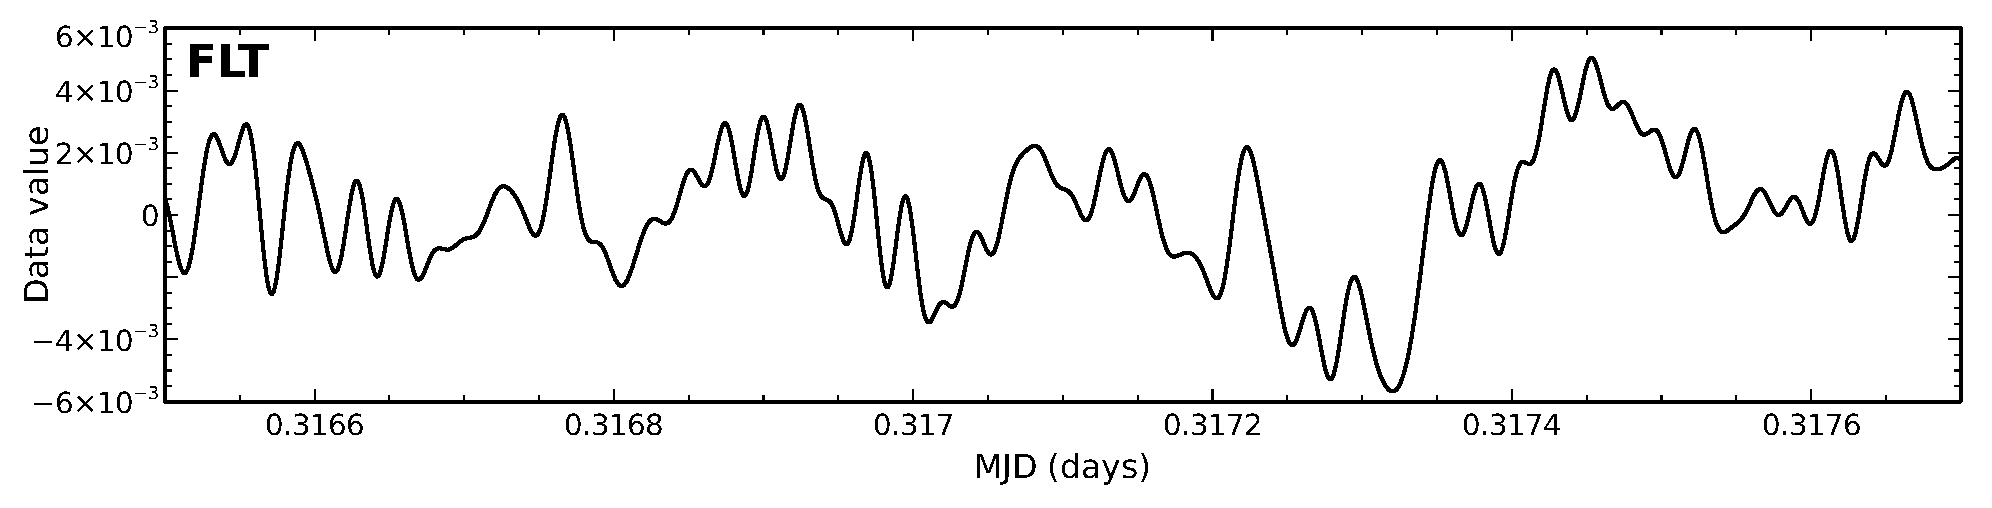
\includegraphics[width=\columnwidth]{flt}
\caption{Maps made with and without FLT model, and the difference between
them. All maps use the same colour scale.}
\label{fig:flt}
\end{figure}


\subsubsection{AST Masking}
\label{sec:astmasking}
AST masking is used to suppress the creation of artificial large scale
background structures in the maps created by \texttt{makemap}. It
consists of forcing background areas in the map to zero after each
iteration. There is some evidence that POL-2 maps made with PCA background
removal are less prone to the creation of these  large scale background
structures than maps made with the standard COM/GAI background removal -
In addition, using AST masking with PCA background removal seems to cause
much slower convergence in \texttt{makemap}. See section~\ref{sec:back}. This
section seeks seeks to investigate these issues.

Four observations of M87 (20160419 \#23, 20160419 \#26, 20160508 \#38
and 20160508 \#41) were reduced without IP correction, without any AST
masking and with PCA background removal. \texttt{makemap} was forced to
perform 40 iterations. At the end of each iteration the FFT of the
current map was taken and the azimuthally averaged spectral power density
found\footnote{The maps were first apodised before taking the FFT, using a
gaussian function that goes to zero at the edge of the valid data. A
constant value was also subtracted from each map to ensure each map has a
zero mean value.}. This is a one-dimensional spectrum showing the strength of
different spatial scales in the map. For each of the four observations,
Fig.~\ref{fig:astmask1} shows a stack of the spectra obtained at the end
of each iteration, green for Q and red for U. Within each stack, the
lowest (weakest) spectrum is for the map created at the end of the first
iteration, and the highest (strongest) spectrum is for the map created at
the end of the last iteration. These stacks illustrate how the strength
of low frequency spatial structures increases strongly with each iteration.

The same thing was done again but using COM/GAI background removal in
place of PCA background removal. The results are shown in
Fig.~\ref{fig:astmask2}. These plots illustrate that the growth of
structures in the range 250 to 500 arc-seconds is much stronger in
maps made with COM/GAI background removal than with PCA background
removal. For 20160419 \#26, large scale structures in the Q map seem to
be 30 times stronger in the COM/GAI maps (peak power \num{12e-5}) than
in the PCA maps (peak power \num{4e-6}). The final Q and U maps for
20160419 \#26 are shown in Fig.~\ref{fig:astmask3}. It is clear that the
COM/GAI maps are far less flat than the PCA Maps - albeit the difference
is not so noticable as the difference in the power spectra would have led
us to expect.

\begin{figure}
\includegraphics[width=\columnwidth]{astmask1}
\caption{Line plots illustrating the growth in the strength of large
scale structures within maps made by consecutive iterations of
\texttt{makemap} using PCA background removal. Green curves are for Q maps and red curves for U maps.}
\label{fig:astmask1}
\end{figure}

\begin{figure}
\includegraphics[width=\columnwidth]{astmask2}
\caption{Line plots illustrating the growth in the strength of large
scale structures within maps made by consecutive iterations of
\texttt{makemap} using COM/GAI background removal.}
\label{fig:astmask2}
\end{figure}

\begin{figure}
\includegraphics[width=\columnwidth]{astmask3}
\caption{The final maps for observation 20160419 \#26. The top row uses
COM/GAI background removal, and the bottom row uses PCA background removal.
The left column holds Q maps, and the right column holds U maps. All maps
use the same colour scale.}
\label{fig:astmask3}
\end{figure}

Whilst PCA background removal seems to reduce the tendancy for large
scale structures to develop, it does not eliminate these structures
altogether. So some means for removing them is still needed. But AST
masking is not ideal as it slows down convergence and produces an
artificially flat background - see Fig.s~\ref{fig:nqu_noast} and
\ref{fig:pcawithast}.

There is an option in \texttt{makemap} to remove large scale changes
between iterations. This option is controlled by the
\texttt{ast.filt\_diff} configuration parameter. The above figures
suggest that the large scale structures are mainly larger than 300
arc-seconds, so another set of maps have been made similar to the ones
described above, but this time with \texttt{ast.filt\_diff=300} in the
\texttt{makemap} configuration. This should suppress the development of
structures larger than 300 arc-seconds. Fig.~\ref{fig:astmask4} shows the
resulting power spectrum stacks, and  Fig.~\ref{fig:astmask5} shows final
Q and U maps. The power in the large scale structures has dropped by more
than a magnitude compared to Fig.~\ref{fig:astmask1}.

\begin{figure}
\includegraphics[width=\columnwidth]{astmask4}
\caption{Line plots illustrating the growth in the strength of large
scale structures within maps made by consecutive iterations of
\texttt{makemap} using PCA background removal with \texttt{ast.filt\_diff=300}.}
\label{fig:astmask4}
\end{figure}

\begin{figure}
\includegraphics[width=\columnwidth]{astmask5}
\caption{The final maps for observation 20160419 \#26 made with
\texttt{ast.filt\_diff=300}. The left image is Q and the right image is U.
These use the same colour scale as the images shown in
Fig.~\ref{fig:astmask3}.}
\label{fig:astmask5}
\end{figure}





\subsubsection{Correction for Instrumental Polarisation}
\label{sec:ip}
Instrumental Polarisation (IP) causes some fraction of the observed total
intensity to become polarised. In other words, some fraction of the total
intensity is converted into Q and/or U by the combination of telescope,
wind-blind and instrumentation, and added onto the intrinsic Q and U
caused by astronomical polarisation. An attempt to estimate and remove
this IP from the observed Q/U time-stream values is made within
\texttt{smurf:makemap} following the initial cleaning process, before the
main iteration loop starts. There is no need for an additional iterative
``model'' to describe IP because the correction does not depend on the
time-stream values and therefore will not change between iterations. The
corrections are based on the total intensity values within a supplied
reference map. This map should cover the same sky area as the observation
being reduced. The default IP correction (named ``PL1'' to distinguish it
from the earlier Johnstone-Kennedy - ``JK'' - model) assumes that the IP
at each point on the sky is an offset in (Q,U) that corresponds to a
vector parallel to the elevation axis, and for which the polarised
intensity is a quadratic function of elevation. It is applied as follows:

\[p = A + B.e + C.e^{2} \]
\[q_{n} = p.cos(-2.e) \]
\[u_{n} = p.sin(-2.e) \]

where $e$ is the boresight elevation in Radians, $p$ is the fractional
polarisation caused by IP, $(q_{n},u_{n})$ are the normalised Q and U
values due to IP (with respect to focal plane Y axis), and $(A,B,C)$ are
constants as follows:

\[A = \num{3.288e-3} \]
\[B = \num{2.178e-2} \]
\[C = \num{-1.156e-2} \]

The above normalised Q and U values are then rotated to use the same
reference direction as the incoming observed Q or U values (\emph{i.e.}
north in the tracking system), multiplied by the corresponding total intensity
in the IP reference map, and then subtracted from the observed Q or U values:

\[Q^{'} = Q - I.( q_{n}.cos(2.\alpha) + u_{n}.sin(2.\alpha) ) \]
\[U^{'} = U - I.( -q_{n}.sin(2.\alpha) + u_{n}.cos(2.\alpha) ) \]

Where $(Q,U)$ are the uncorrected observed Q and U values at some point
on the sky, $(Q^{'},U^{'})$ are the corrected observed Q and U values,
$I$ is the total intensity at the same point on the sky (taken from the
IP reference map), and $\alpha$ is the angle from the reference direction
used by the $(Q,U)$ values  to the focal plane Y axis, measured positive
in the sense of rotation from focal plane Y to focal plane X. The $I$
value is determined by nearest neighbour interpolation. That is, $I$ is
the value of the pixel within the IP reference map that contains the
sky position corresponding to the $(Q,U)$ time-stream sample.

Note, any noise present within the IP reference map will be transferred
directly by the above process into the final Q and U maps, and so it seems
a good idea to use a low noise IP reference map. However, the IP is at
around the 1 \% level  (\emph{i.e.} $p$ in the above equations is around
0.01) and so only around 1 \% of the noise in the IP reference map will
be transferred into the Q and U maps.

Correction for IP could instead be applied to the final Q and U maps,
rather than being applied to the time-stream values that go into the
map-making process. However, for a long observation the elevation (and
therefore the IP) of the samples that fall in any one map pixel can
change significantly over the course of the observation. It was therefore
considered better to apply the IP correction to the Q/U time-streams
rather than the resulting Q/U maps.

There are two potentially problematic issues remaining with the basic IP
correction described above: 1) difference in the beam shape between the IP
reference map and the actual IP, and 2) differences in the spatial frequencies
present in the IP reference map compared to the resulting POL-2 maps. These
are described further below.

\paragraph{The IP beam shape}
The ``PL1'' IP model is based on observations of unpolarised planets (hence
the name - the first planet IP model). Specifically, it is based on 31
observations of Uranus obtained in October and November 2015 over a wide
range of elevation and azimuth. Polarised intensity maps made from these
observations show a beam shape that varies with elevation. The main beam tends
to be elliptical, with ellipticities that vary from 1.1 at 20$^\circ$
elevation to 1.6 at 75$^\circ$. The major axis of the elliptical beam
seems to be roughly parallel to azimuth at all elevations. The cause of
this non-circular beam shape is discussed else where in this commissioning
report.  However, the basic IP correction method described above does not
take this beam shape into account. In general the IP reference map will
be a standard SCUBA-2 map and so will have the standard SCUBA-2 beam shape,
which is circular. Thus the IP correction will have a circular beam shape
and will not in general match the elliptical beam shape of the actual IP in
the observed $(Q,U)$ values. The correction will therefore leave areas of
systematically positive or negative residuals around point sources. This
section describes how the IP reference map can be modified so that it has
a beam shape that is close to the observed elliptical IP beam shape. The
first task is to characterise the IP beam shape so that we can generated an
expected beam shape at any elevation. Then we need to modify the IP
reference map so that it has the IP beam shape expected at the elevation
of the observation being corrected. Then we need to test the effects of
modifying the IP reference map in this way:

\begin{itemize}
\item {\bf Characterising the IP beam shape:}
Fig.~\ref{fig:ip1} shows the measured shape and size of the IP beam over
a range of elevations, together with quadratic fits to these properties.
The observations used were the set of 31 Uranus observations that were
used to create the PL1 IP model. The beam properties were found using
\texttt{kappa:beamfit} to fit to the polarised intensity image of
Uranus in each map. The fits allow the expected beam shape and size at any
elevation to be estimated.

\begin{figure}
\includegraphics[width=\columnwidth]{ip1}
\caption{The parameters of the IP beam shape at different elevations and
azimuth. The red dots indicated measured values calculated using
\texttt{kappa:beamfit}, and the blue dots indicate quadratic fits to the
red dots.}
\label{fig:ip1}
\end{figure}

\item {\bf Modifying the IP reference map:}
Ideally, in order to minimise residuals in the IP correction we would
like the total intensity map to have the same beam shape as the
IP-generated polarised intensity. In principle we could achieve this by
first deconvolving the total intensity map using its own beam as the PSF,
and then convolving the resulting map using the IP beam as the PSF. So if
$I$ is the total intensity map with circular beam $B_{I}$ and $I_{0}$ is
the high resolution ``true''" total intensity map, then:

\[ I = I_{0} \otimes B_{I} \]

where $\otimes$ is the convolution operator. Also, if $I_{ip}$ is the required
total intensity map with beam $B_{ip}$ (the IP beam), then:

\[ I_{ip} = I_{0} \otimes B_{ip} \]

What we want is some convolution kernel, $K$, with which we can smooth the
original total intensity map, $I$, in order to create the required total
intensity map, $I_{ip}$. In other words, we want $K$ where:

\[ I_{ip} = I \otimes K\qquad .\ .\ .\ .\ .\ (1)\]

Substituting for $I$ and $I_{ip}$ using the earlier expressions gives:

\[ I_{0} \otimes B_{ip} = ( I_{0} \otimes B_{I} ) \otimes K \]

Since convolution is commutative and associative, we can rearrange this to:

\[ I_{0} \otimes B_{ip} = I_{0} \otimes ( K \otimes B_{i} ) \]

and so

\[ B_{ip} = K \otimes B_{I} \]

In other words, smoothing $K$ using the original circular I beam gives you
the elliptical IP beam. The corollary of this is that deconvolving the
elliptical IP beam using the circular I beam must give you $K$.

Image deconvolution in the presence of noise is a very tricky business.
To simplify things, \texttt{kappa:beamfit} is used first to fit a Gaussian-like
function to Uranus in the total intensity map and then this noise-free
model is used as the $B_{I}$ image above. The $B_{ip}$ image (the IP beam
shape) varies with azimuth and elevation and is generated from an analytical
expression as follows based on the fits to the IP beam parameters shown in
Fig.~\ref{fig:ip1}:

\[ B_{ip} = e^{ -4.ln(2).\left( \left( \frac{u}{fu} \right)^{2} +
\left( \frac{v}{fv} \right)^{2}\right)^{\frac{g}{2}}} \]
\[ u = x.sin(\alpha) + y.cos(\alpha) \]
\[ v = -x.cos(\alpha) + y.sin(\alpha) \]

Here, $x$ and $y$ are the pixel coordinates within the $B_{ip}$ image. The
shape of the beam is determined by the constants $\alpha$, $fu$, $fv$ and
$g$, all of which are functions of azimuth or elevation and are determined
using the fits described in the previous section. Specifically, $\alpha$
is the angle from the elevation axis (i.e. the Y pixel axis) to the major axis of the
elliptical beam, $fu$ and $fv$ are the major and minor FWHM beam sizes
(in pixels), and $g$ is the exponential power (i.e. 2.0 for a Gaussian).

Having obtained the $B_{I}$ and $B_{ip}$ images, the required kernel $K$
is found by deconvolving $B_{ip}$ using $B_{I}$ as the PSF. KAPPA provides
three ways of doing deconvolution; basic division in Fourier space, a
Wiener filter, or the Richardson-Lucy algorithm (sadly, KAPPA no longer
contains the MEM2D maximum entropy deconvolution command). All three were
tried and the Wiener filter option produced the most usable results.

Two final modifications to the kernel are performed. As is commonly seen
in Wiener deconvolutions, rings are visible around bright sources in the
final $I_{ip}$ map if $K$ is used unmodified. These rings are reduced if the
kernel $K$ is apodised before being used - \emph{i.e.} a windowing function is
applied to the kernel that causes it to drop off to zero more quickly
with increasing distance from the centre. The windowing function used is
a simple circular Gaussian with a peak value of 1.0 and an FWHM of 30
arc-seconds. The second modification is to ensure the kernel has a total
data sum of 1.0. This is necessary to ensure that the resulting $I_{ip}$ map
has the same normalisation as the original I map.

The whole process can be tested by using equation $(1)$ above to generate
a total intensity map of Uranus with the beam shape expected for the IP
at a chosen elevation, and then compare the resulting image with the
actual IP beam shape seen at the same elevation. Fig.~\ref{fig:ip2},
does this for a single observation. It can be seen that visually, the beam
in the central image - the modified IP reference map - is similar to that
in the right image - the actual IP beam at the same elevation. Both are
extended by about the same amount parallel to the azimuth axis. Faint
rings are visible around the source in the central image, but these
are much worse without the apodising described above.

Using \texttt{kappa:beamfit} to measure the shape of the beam in the
centre and right images gives:

\begin{tabular}{l|c|r}
  Property & Centre image value & Right image value \\
  \hline
  FWHM1 & 17.0$"$ & 15.9$"$ \\
  FWHM2 & 12.3$"$ & 12.1$"$ \\
  Angle (w.r.t. elevation) & 94$^{\circ}$ & 15.9$^{\circ}$ \\
  Exponential power & 2.2 & 2.6 \\
\end{tabular}

So the attempt to change the beam shape in the total intensity reference
image so that it matches the IP beam at the same elevation is working -
roughly but not perfectly. Even though it is not perfect it should
produce an improvement in the residuals left after IP correction of the
Uranus maps.

\begin{figure}
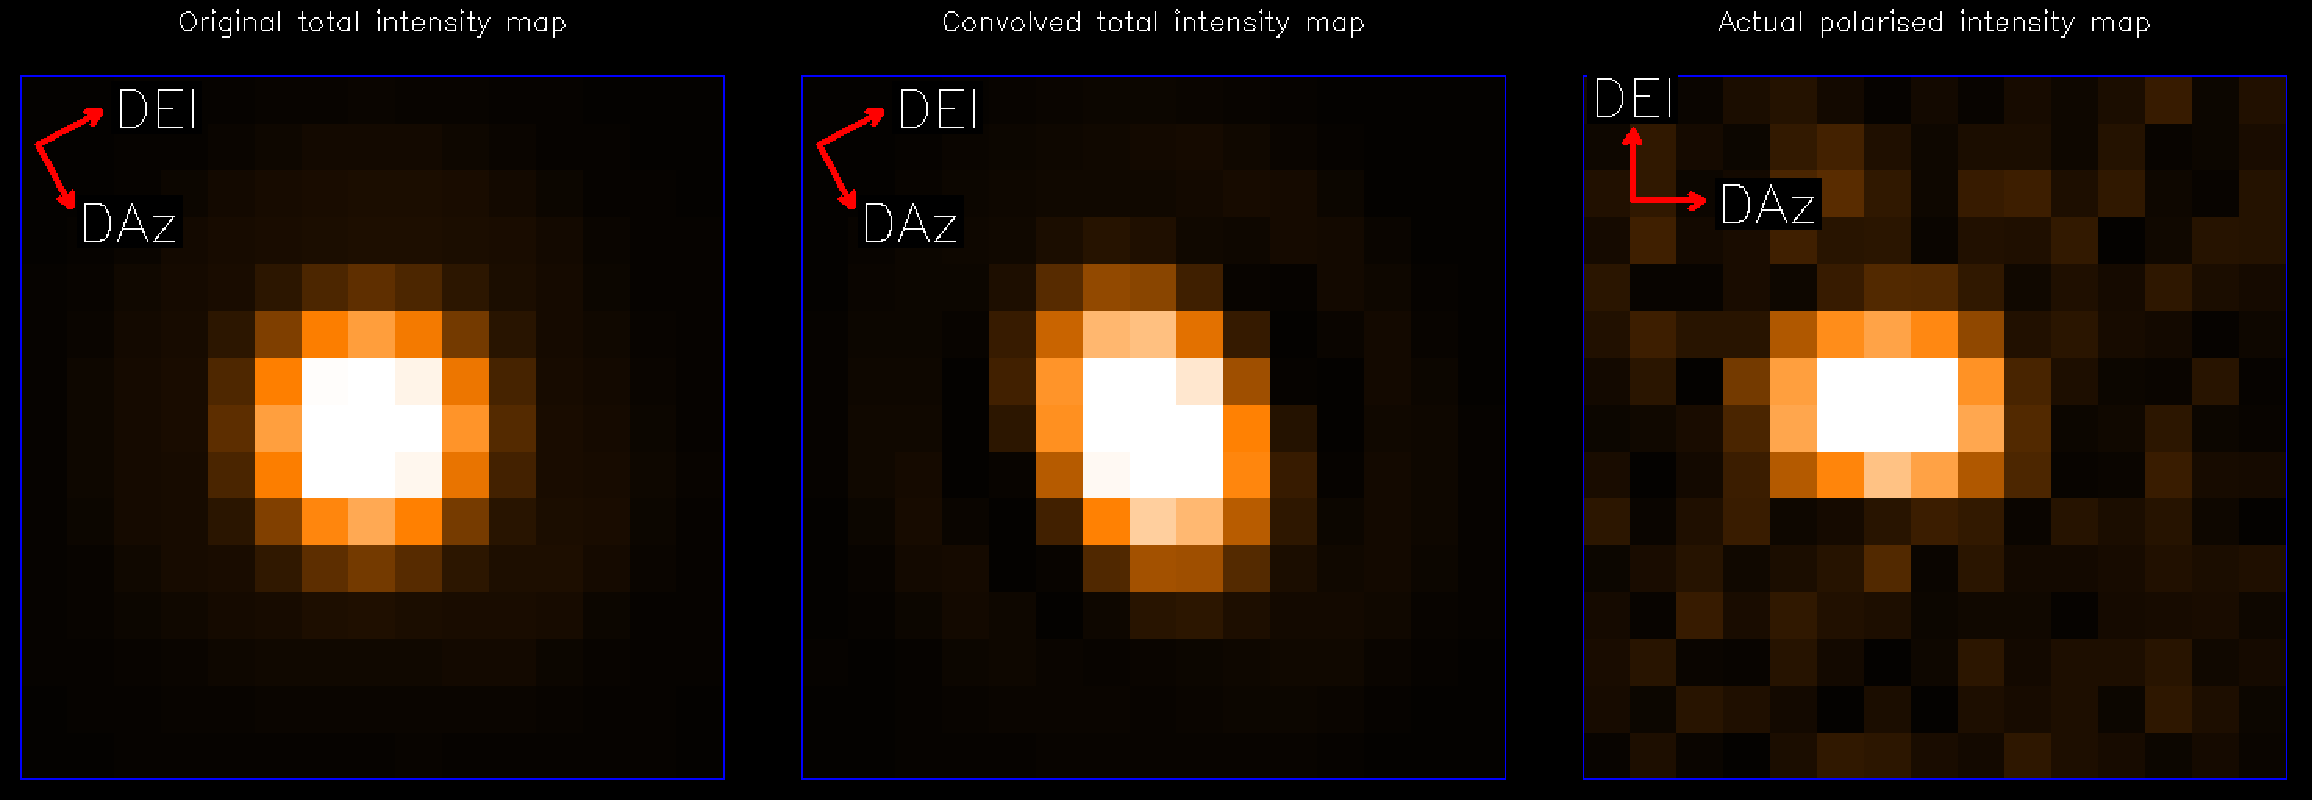
\includegraphics[width=\columnwidth]{ip2}
\caption{Convolving a circular beam map of Uranus to match the IP beam.
The left hand image is the original total intensity map of Uranus, the
right hand image is the polarised intensity map created from observation
67 on 20151007 (elevation 36$^{\circ}$), and the central image is the
total intensity map created by convolving the left hand image with the
$K$ kernel. The left hand two images use the same grey scale.}
\label{fig:ip2}
\end{figure}

\item {\bf Verifying the effects of the modified IP reference map:}
The 31 Uranus observations were re-reduced with IP correction. With
perfect IP correction this would result in Q and U maps containing just
noise. The nature of the residual Q and U signal indicates the success
of the IP correction. Fig.~\ref{fig:ip3} compares maps made with no IP
correction, basic IP correction and the modified IP correction described
above. The modified IP correction is clearly producing a good effect in
these two observations.

\begin{figure}
\includegraphics[width=\columnwidth]{ip3}
\caption{Applying IP correction to Q/U maps of Uranus. Top row show Q
maps for observation 26 on 20161007. Bottom row shows U maps for
observation 57 on 20161007. Left images show Q or U without any IP
correction, middle images shows the Q or U with basic IP correction
(\emph{i.e.} without the beam shape fix), and right images shows
the IP-corrected Q or U with the beam shape fix. The three images in
a row use the same grey scale. }
\label{fig:ip3}
\end{figure}

To measure the improvement produced by the beam correction, the standard
deviation of the Q or U values over a 40 arc-sec diameter aperture
centred on the source is found, in both the original (basic IP
correction) and fixed (modified IP correction) Q and U maps, and the
ratio is formed. Fig.~\ref{fig:ip4} shows the ratio:

\[ \frac{standard\ deviation\ of\ Q\ or\ U\ values\ without\ fix}{standard\ deviation\ of\ Q\ or\ U\ values\ with\ fix} \]

plotted against elevation. In other words, values larger than one
indicate that the fix is doing some good. These plots make it clear that
the fix is more beneficial in places where the instrumental Q or U is
stronger (Q is strong at high and low elevation, and weak at mid
elevations, U is strong at mid elevations and weak at high and low
elevations).

\begin{figure}
\includegraphics[width=\columnwidth]{ip4}
\caption{Improvement in residuals produced by the modified IP correction.
The left hand plot is for Q and the right hand plot for U.}
\label{fig:ip4}
\end{figure}

In terms of its effect on maps of polarised sources, the correction seems
to make little if any change. There is a marginal improvement in the
shape of 3C273 within a co-add of 13 U maps, as show in Fig.\ref{fig:ip5}.
The map made with basic IP correction has an aspect ratio of 1.4
(determined by \texttt{kappa:beamfit}, and the map made with modified IP
correction has an aspect ratio of 1.15. So the map made with the beam-shape
fix is slightly  less elliptical.

\begin{figure}
\includegraphics[width=\columnwidth]{ip5}
\caption{Effects of modified IP correction on a co-add of 13 U maps of
3C273. Left image is made with basic IP correction. Right image is made
with modified IP correction.}
\label{fig:ip5}
\end{figure}

\end{itemize}

The above IP beam shape correction is implemented as an option within the
\texttt{smurf:pol2scan} command - a Python script that modifies the
supplied IP reference map as described above and then invokes \texttt{makemap},
passing it the modified IP reference map. By default, the option is off,
meaning that basic IP correction is used.

\paragraph{Spatial frequencies present in the IP map}
As described above, IP correction is performed by scaling a supplied
total intensity reference map and then subtracting it from the original Q
or U time-stream values before converting them into a map. The aim
obviously is that the IP estimated from the reference map should cancel
out the actual IP present in the data. However, if the reference map
contains any features that are not present in the POL-2 data, these will
not be cancelled out and will appear in negated form within the final Q
or U map.

For instance, if the IP reference map contains spatial frequencies that
are not present in the POL-2 data, these spatial frequencies will pollute
the final Q and U maps. The spatial frequencies present in the IP
reference map will depend on the scanning mode and the map-maker
configuration with which it was made, and so may be quite different to
the spatial frequencies present in the POL-2 data. As yet, the
consequences of using different IP reference maps have not been
investigated. This should be done at some point, maybe using simulated
POL-2 data for a known sky map to estimate the size of any effects.

Note however that the IP correction is done on the Q/U time-streams prior
to converting them into a map, so the spatial filtering produced by the
iterative map-making process will be applied in the same way to both the
original Q/U values and to the Q/U correction values sampled from the IP
reference map. The situation would almost certainly be worse if the IP
correction was instead applied to the final Q/U maps.

\subsubsection{Correction for pointing errors}
Polarised intensity maps made from POL-2 observations demonstrate random
pointing errors. These pointing errors can cause mis-alignment between the
Q/U time-stream data and the reference map used for IP correction (see
section~\ref{sec:ip} for details of IP correction). This in turn can cause
spurious features to appear around bright, weakly polarised point
sources, for which the IP correction is more significant. The size of
these pointing errors seems to be comparable with other non POL-2
observations - typically less than 3 arc-seconds but occasionally reaching
values as high as 8-10 arc-seconds.

That these pointing errors are intrinsic to the telescope and/or data
acquisition, and not caused by the data reduction, can be seen by
comparing the centroid positions within polarised intensity maps of
Uranus, created using the procedure described above, with the centroid
positions within total intensity maps made by running the raw analysed
intensity data through \texttt{makemap} directly, without first using
\texttt{calcqu} to create Q/U time streams.

31 observations of Uranus were reduced again, without IP correction, and
with 4 arc-sec pixels, using focal plane Y as the reference direction.
The position of Uranus in each observation was found in three different ways:

\begin{enumerate}
\item Finding the centroid of the emission around the source within the de-biased
polarised intensity maps
\item Finding the centroid of the emission around the source within the total
intensity maps made from the total-intensity time streams generated by
\texttt{calcqu}, using COM/GAI background subtraction within \texttt{makemap}.
\item Finding the centroid of the emission around the source within the total
intensity maps made by processing the raw analysed intensity time streams
directly using \texttt{makemap} with COM/GAI background subtraction.
\end{enumerate}

Fig.~\ref{fig:point1} compares the X and Y positions found using these
methods. The left plot shows centroid X axis values and the right plot
shows centroid Y axis values, all in pixels. In both cases, the
horizontal axis represents the third of the above three centroid
positions, and the vertical axis represents the first (red) and second(
blue) centroid positions.

\begin{figure}
\includegraphics[width=\columnwidth]{point1}
\caption{Comparing pointing errors within maps of Uranus created by
three different methods.}
\label{fig:point1}
\end{figure}

The scatter on the red spots (method 1) is greater than the blue because
the polarised intensity is much weaker than the total intensity, and so
the error on the centroid position is greater. But otherwise these plots
show that the positional errors using method 3 - which does not use
\texttt{calcqu} or PCA background removal within \texttt{makemap} -
are basically the same as for the other two methods. So the positional
error is unlikely to be caused by \texttt{calcqu} or the PCA background
removal.

As mentioned above, the typical sizes of these pointing errors are
consistent with other non-POL-2 observations. However, when a large error
occurs it may cause problems for bright, weakly polarised point sources
due to mis-alignment with the IP reference map. For this reason, the
\texttt{smurf:pol2scan} command includes a form of pointing correction,
which works as follows:

\begin{itemize}
\item When \texttt{calcqu} is run to create Q and U time-streams from the
original analysed intensity time streams, it also creates a total
intensity ($I$) time-stream sampled at the same rate as the Q and U
time-streams. These $I$ values are the background values at the
centre of each fit in the original analysed intensity time streams (see
section~\ref{sec:fit}).
\item This $I$ time-stream is converted into an $I$ map using \texttt{makemap}
(with no pointing corrections).
\item Any mis-alignment between this $I$ map and the supplied IP reference
map is then measured using \texttt{kappa:align2d}.
\item \texttt{makemap} is then used to create maps from the Q and U
time-streams, applying corrections for any misalignment identified in the previous
step. These corrections modify the position of each Q/U sample on the sky
before they are binned into a map, thus avoiding the need to re-sample the
final maps.
\end{itemize}

The final alignment is not perfect due to limitations in the
\texttt{kappa:beamfit} command. However, the above pointing correction
certainly improves the alignment of multiple maps, reducing pointing
errors typically by 50\%.

\subsubsection{Standard POL-2 \emph{dimmconfig} files}
SMURF includes three ``dimmconfig'' files that specify \texttt{makemap}
configurations specific to POL-2 data. These are stored in the standard
location (\texttt{\$STARLINK\_DIR/share/smurf}) and are described below:

\paragraph{\texttt{.dimmconfig\_pol2.lis}}
This is a \emph{hidden} file (\emph{i.e.} the name starts with a dot)
because it is not intended to be used directly by user. Instead, it is
intended to be used as the basis for other POL-2 dimmconfig files. It
sets the following configuration parameters values (all others retain the
defaults values set in \texttt{\$SMURF\_DIR/smurf\_makemap.def},
\emph{etc.}):

\begin{quote}
\begin{description}

\item[\texttt{modelorder=(pca,ext,ast,noi)}] This causes common-mode backgrounds
to be removed from the Q/U time-streams using the PCA model rather than
the default COM/GAI model. See section~\ref{sec:back}.

\item[\texttt{spikethresh=5}] Enable spike detection and removal within the Q/U
time-streams during the cleaning phase, prior to the start of the
iterative algorithm. This is done because polarised sources can be very
faint, thus requiring very few iterations (sometimes only one iteration is
needed). This means that the default map-based de-spiking is less
effective. Map-based de-spiking is retained, but is aided by also enabling
time-based de-spiking. The value of 5 is the threshold, in units of
standard deviations, at which to flag spikes within the time streams.
Time-based de-spiking was broken in \texttt{makemap} before 11th June
2015 (git commit 0e8d37602), which is why it is not used in most SCUBA-2
dimmconfig files.

\item[\texttt{spikebox=10}] The default box size of 50 samples for time-based
de-spiking is far too high because of the very slow sample rate in Q/U
time-streams.

\item[\texttt{flagslow=0.01}] The lowest usable telescope speed. The default value
of 30 arc-seconds per second is inappropriate for POL-2 because of the
very low scan speed. This over-ride sets it to 0.01 arc-seconds per
second - which is probably lower than it needs to be. See
section~\ref{sec:slow}.

\item[\texttt{noisecliphigh=3}] The threshold (in standard deviations) at which to
reject noisy bolometers. The default value is 4. Setting it to 3
(\emph{i.e.} reject more bolometers) seems to produce marginally better
maps.

\item[\texttt{downsampscale=0}] Prevent any further down-sampling of the Q and U
time-streams. The \texttt{calcqu} command down-samples the time streams
from a nominal 175 Hz to 2 Hz, so no further down-sampling is needed.

\item[\texttt{noi.usevar=1}] This affects the weight used for each Q/U
time-stream sample when they are binned into the final map using a
weighted mean estimator. By default, the weights are derived from the
power in the 2-10 Hz band. This in inappropriate for Q/U time streams
because of their very low sample rate. Setting \texttt{noi.usevar=1}
causes the weights to be derived from the Variance values stored in the
supplied Q/U input NDFs. These are created by \texttt{calcqu} and are related
to the RMS residual in the fitting box from which the Q or U value was
found (see section~\ref{sec:fit}).

\end{description}
\end{quote}


\paragraph{\texttt{dimmconfig\_pol2\_compact.lis}}
This is intended for observations of compact sources (less than 60
arc-seconds in radius). It inherits all the settings in
\texttt{.dimmconfig\_pol2.lis} described above, and adds:

\begin{quote}
\begin{description}

\item[\texttt{ast.zero\_circle=0.016}] This causes AST masking to be used,
where the source is defined by a circle of radius 60 arc-seconds centred
on the expected source position. All pixel values outside this circle are
forced to zero at the end of every iteration, except for the last
iteration. This is intended to prevent the development of artificial
large scale background structures. However, this setting may not be
necessary since such structures tend to take many iterations to develop,
and POL-2 maps usually require relatively few iterations to converge
because of the faintness of most sources in polarised intensity.
Also, the PCA background removal used with POL-2 data seems to be more
resilient against such structures than the usual COM/GAI background
removal. See section~\ref{sec:back}.

\end{description}
\end{quote}

\paragraph{\texttt{dimmconfig\_pol2\_extended.lis}}
This is intended for observations of extended sources. It inherits all the
settings in \texttt{.dimmconfig\_pol2.lis} described above, and adds:

\begin{quote}
\begin{description}

\item[\texttt{ast.zero\_snr=3}] This causes AST masking to be used,
where the source is defined by an SNR threshold of 3. All pixel values
below this SNR threshold are forced to zero at the end of every iteration,
except for the last iteration. This is intended to prevent the development
of artificial large scale background structures. However, this setting may
not be necessary since such structures tend to take many iterations to
develop, and POL-2 maps usually require relatively few iterations to
converge because of the faintness of most sources in polarised intensity.
Also, the PCA background removal used with POL-2 data seems to be more
resilient against such structures than the usual COM/GAI background
removal. See section~\ref{sec:back}.

\item[\texttt{ast.zero\_snrlo=2}] This causes each contiguous area within
the AST masking defined by the previous setting to be extended down to
an SNR of 2. It also causes small isolated ``islands'' of a few high-SNR
pixels to be excluded from the AST mask.

\item[\texttt{numiter=-40}] This allows up to 40 iterations to be
performed when making the map. The default is 5 iterations. There is some
evidence that using AST making seriously raises the number of iterations
needed for convergence.  See section~\ref{sec:back}.

\end{description}
\end{quote}

Note, unlike file \texttt{dimmconfig\_bright\_extended.lis}, no value is
set for \texttt{ast.skip}. This is because no FLT model is used, and
therefore we do not need to reserve any initial iterations for determining
a FLT mask in order to reduce bowling around sources.


\subsubsection{Reference direction}
By default, the Q and U values created by \texttt{smurf:calcqu} are
specified with respect to a reference direction which is parallel to
north in the selected tracking system\footnote{Optionally, they may
instead use the focal plane Y axis as the reference direction.}.
Positive polarisation angles are in the same sense as rotation from the
focal plane X axis to the focal plane Y axis. \texttt{makemap} bins the
supplied Q or U values into pixels directly, without any change to the
reference direction. So the Q and U maps created my \texttt{makemap} also
use tracking north as the polarimetric reference direction. This means
that the orientation of the reference direction with respect to the pixel axes
may change across the map. For instance, if the north pole was at the
centre of the map then the polarimetric reference direction at any pixel
would be a radial line pointing to the centre of the map.

The WCS FrameSet stored in each Q or U map created by \texttt{makemap} will
include a Frame with Domain ``POLANAL''. The first axis of this Frame
defines the polarimetric reference direction, and consequently will
usually be parallel to tracking north. The POLANAL Frame is used by
commands within the POLPACK package (see SUN/223) and is also used by the
polarimetry toolbox within the GAIA display tool (see SUN/214). The
\texttt{polpack:polrotref} command can be used to modify the polarimetric
reference direction within a pair of corresponding Q and U maps.

\subsubsection{Using SkyLoop with POL-2 data}
\label{sec:skyloop}
Faint astronomical sources will have very low polarised intensity, and
consequently it is common to combine multiple observations to create the
final Q and U maps. For non-POL-2 observations, using the
\texttt{smurf:skyloop} command has been shown sometimes to produce better
results for faint sources than simply running \texttt{smurf:makemap} on
each observation and the co-adding the resulting individual maps.
Experiments should be made to see if this also true from POL-2 data.

The \texttt{smurf:pol2scan} command currently has no option to use
\texttt{skyloop} instead of \texttt{makemap}. To use \texttt{skyloop} it
is therefore necessary to run the individual commands manually. For
instance:

\begin{verbatim}
   % mkdir qudir
   % calcqu in=$SC2/s8\?/20160508/00041/\* outq=qudir/\*_QT outu=qudir/\*_UT
   % skyloop in=qudir/\*_QT out=qmap ref=m87 ipref=m87 pixsize=4 \
        config=^$STARLINK_DIR/share/smurf/dimmconfig_bright_extended.lis
\end{verbatim}

\section{Creation of vector catalogues}
\label{sec:vectors}
The \texttt{smurf:pol2scan} command creates Q and U maps from the raw
analysed intensity data for a single POL-2 observation by running
\texttt{smurf:calcqu} followed by \texttt{smurf:makemap}. In addition, it
can also use the resulting Q and U maps to create a catalogue of
polarisation vectors in FITS binary table format (see the CAT parameter
in the documentation for \texttt{pol2scan} - SUN/258). Often it will be
required to co-add multiple POL-2 observations before creating a
catalogue. This can be done using the \texttt{smurf:pol2stack} command,
which accepts a list of existing Q, U and I maps as input, and creates
co-added Q, U and I maps together with a vector catalogue as outputs.

\texttt{pol2stack} aligns the input maps first if required, and modifies
them so that the Q and U maps use the same polarimetric reference
direction (using \texttt{polpack:polrotref}). They are then co-added to
create master Q, U and I maps. The \texttt{polpack:polvec} command is
then used to create a a vector catalogue from these master maps in FITS
binary table format. See the documentation for \texttt{polpack:polvec}
(SUN/223) for a list of the columns in this catalogue.

\begin{quote}
\emph{Note, the reliability of the uncertainties on polarisation and angle
in these catalogues is still under investigation. The statistics of these
quantities are complicated because of the non-linear calculations needed
to create them. It is often safer to look at the Q and U maps - which
have much simpler statistics - when assessing the significance of any
feature within the vector map.}
\end{quote}

Four POL-2 observations of CB 68 were co-added and a vector catalogue
created. Then an additional three observations were obtained and the
resulting list of seven observations were co-added and a second vector
catalogue created. For each position, the ratio of the error on the angle
in the seven-observation catalogue to the error on the angle in the
four-observation catalogue was formed. It is expected that the extra
integration time will reduce the errors, thus the above ratio values
should be smaller than unity. Fig.~\ref{fig:error1} shows a histogram of
the ratio values. Only values within the central 2.5 arc-minute box that
have angle errors less than 50 degrees were included. The mean value is
1.2, which is bad in so far as it suggests that the noise has gone up
rather than down, but it is a consequence of the heavily skewed
distribution. The peak value in the histogram (0.8) is less than one and
indicates a reduction in the noise comparable to that expected from the
increased exposure time (0.78).

The similar histogram shown in Fig.~\ref{fig:error2} was formed in the
same way, but the two catalogues were first binned into $12x12$
arc-second bins (this is a $3x3$ pixel box within the original un-binned
catalogue) before selecting the vectors. The binning was done using
\texttt{polpack:polbin}, which finds the mean Q, U and I value in each
bin and then re-calculates the vector angle and polarisation from the
binned values. This histogram does not have the smooth shape of the
histogram in Fig.~\ref{fig:error1}. The peak value is less well defined
and occurs at a value of 1.0, indicating that the additional three observations
are now not improving the errors on the angle.

It is not clear why binning the catalogues should cause this change in
the catalogue. Further investigation is needed. Also, several people have
commented that the error on percentage polarisation seem unrealistically
low for vectors within the faint outer regions of extended source. For
instance Jia-Wei Wang found this when looking at a vector catalogue
produced for the BISTRO Ophiuchus L 1688 field1 (20160422\_00053,
20160424\_00016, and 20160424\_00033).

\begin{figure}
\includegraphics[width=\columnwidth]{error1}
\caption{A histogram of the fractional reduction in error on angle
as a result of adding in an extra three observations into a four
observation co-add of CB 68.}
\label{fig:error1}
\end{figure}

\begin{figure}
\includegraphics[width=\columnwidth]{error2}
\caption{Shows the same data as Fig.~\ref{fig:error1}, but in this case
the data has been binned up prior to selecting the vectors to be included
in the histogram.}
\label{fig:error2}
\end{figure}

\section{Display and analysis of vector catalogues}

\subsection{Display and analysis using GAIA}

The polarimetry toolbox within GAIA (SUN/214) can be used to display and
explore vector catalogues. A typical screen-shot is shown in
Fig.~\ref{fig:gaia}. Features include:

\begin{enumerate}
\item display a vector map over a total intensity image.
\item change the scale and density of the displayed vectors.
\item select vectors either on the basis their position, or on the basis
of the catalogue values.
\item display statistics of the selected vectors.
\item remove selected vectors form the catalogue.
\item bin the catalogue to produce fewer vectors.
\end{enumerate}

\begin{figure}
\includegraphics[width=\columnwidth]{gaia}
\caption{The GAIA image display displaying a vector map. The displayed
dialogue box contains the polarimetry toolbox.}
\label{fig:gaia}
\end{figure}

To use it, start up gaia specifying the total intensity map on the
command line:

\begin{quote}
\begin{verbatim}
% gaia imap.sdf
\end{verbatim}
\end{quote}

Then select ``Polarimetry toolbox...'' from the ``Image-Analysis'' item
on the menu bar. This pops up a new dialogue box. Within this box, click
on ``Open'' within the ``File'' menu, and select the disk file holding
the vector catalogue to be displayed (it will usually have a file suffix
of \texttt{.FIT}). The vectors will be plotted over the total intensity
map with some default scale, and a table of the catalogue columns will be
displayed in the dialogue box. Further help is available by clicking on
the ``help'' menu button. Hovering the pointer over any control will
cause a description of the control to appear in the status bar at the
bottom of the dialogue box.

Usually, the first thing to do is to select and remove bad vectors (these
will often cause an inappropriate default vector scale to be used). This
can be done by clicking on the tab labelled ``selecting'' on the left
hand side of the dialogue box. An expression describing the bad vectors
should be entered into the ``Expression'' box, and the return key should
then be pressed. A suitable expression may be:

\begin{quote}
\begin{verbatim}
$p>50 || $dp>10 || $dang>50
\end{verbatim}
\end{quote}

This selects any vectors that have polarisation ($p$) greater than 50
\%, or have an polarisation uncertainty ($dp$) greater than 10 \%, or have an
uncertainty in the vector angle ($dang$) greater than $50^{\circ}$.
Vectors can also be selected by clicking and dragging out a box on the
main gaia window. These selected vectors can then be removed by clicking
``Cut'' within the ``Edit'' menu (keyboard short-cut \texttt{Control-X}).
This will remove the selected vectors from both the table and the vector
map. The vector scale should then be reset by clearing the ``Vector
scale'' box on the ``Rendering'' tab, and then pressing return (this
forces the calculation of a new default vector scale on the basis of the
remaining vectors). Alternatively, an explicit scale value can be entered
into the box (do not forget to press return after typing the value). The
display can be panned and zoomed as normal using the controls in the main
GAIA window in order to see more detail.

You may also want to display a binned-up vector map. This can be done
using the controls on the ``Binning'' tab. Enter the required box size
(given as a number of map pixels) and then press the ``pointing hand''
button to bin the catalogue and display the result.

Statistics for the \emph{selected} vectors can be viewed on the
``Statistics'' tab (note, no statistics will be displayed if no vectors
are currently selected).

The catalogue columns that define the length and orientation of each
vector can be selected on the ``Rendering'' tab.

If you hover the pointer over a vector, it will be high-lighted by a
change of colour and its length will be displayed next to the vector.
Clicking on the vector will highlight the corresponding row in the table.
Conversely, clicking on a row in the table will highlight the
corresponding vector on the main display.

The currently displayed catalogue can be saved in a new file using the
``Save as'' item in the ``File'' menu of the dialogue box. The saved
catalogue will incorporate any changes made to the catalogue using
the methods describe above (\emph{e.g.} removal of selected vectors or
binning of the catalogue).

\subsection{POLPACK and KAPPA}
The GAIA tool is very useful for interactive exploration of a catalogue,
but it is currently difficult to save the visual appearance of the map. The
only successful method seems to be to use an external screen-shot tool such
as \texttt{ksnapshot} (provided as part of KDE) or some equivalent.

For printed output, the \texttt{polpack:polplot} command can be used to
plot the vector map, in conjunction with other commands such as
\texttt{kappa:display}, \texttt{kappa:picdef}, \texttt{kappa:picsel} to
display the underlying total intensity map.

A useful approach is often to do the initial investigation in GAIA,
possibly removing bad vectors and binning-up the catalogue. Save the
modified catalogue in GAIA using the ``Save as'' item in the ``File''
menu of the polarimetry toolbox and then display the modified catalogue
for printing using POLPACK and KAPPA.

KAPPA and POLPACK can produce graphics using a variety of graphics
devices. The two most useful are ``xwindows'' (a visible window on your
computer) and ``Accumulating Postscript'' (where the graphics output from
consecutive commands are accumulated into a single postscript file - named
\texttt{pgplot.ps} by default). All graphics output goes to the current
device, which can be selected using the \texttt{kappa:gdset} command:

\begin{quote}
\begin{verbatim}
% gdset xw
% gdset apscol_p
\end{verbatim}
\end{quote}

The first example above selects xwindows and the second selects
accumulating postscript (colour, portrait mode). It is often a good idea
to prototype your plot using xwindows, and then change to accumulating
postscript to produce the final \texttt{.ps} file\footnote{Postscript
files can be converted to PDF using commands such as \texttt{ps2pdf}.}.
My options are available to control how the plotting surface is divided
up into separate pictures and how each picture appears. For more details
see the KAPPA documentation (SUN/95 - especially sections ``Graphics
Devices and Files'', ``Plotting Styles and Attributes'' and ``The
Graphics Database''), and the POLPACK documentation (SUN/223 - especially
section ``Displaying the Results''). The following example C-shell script
illustrates just a few of the available options. It produces the output
shown in Fig.\ref{fig:myplot}.

\begin{figure}
\includegraphics[width=\columnwidth]{myplot}
\caption{A composite plot produced using KAPPA and POLPACK.}
\label{fig:myplot}
\end{figure}

\begin{quote}
\begin{verbatim}

#  Start up the required Starlink packages
kappa
polpack

#  Use a postscript font rather than a native PGPLOT font.
setenv PGPLOT_PS_FONT Helvetica

#  Select the accumulating postscript graphics device, and clear any
#  current pictures in the graphics database. All output will go to file
#  pgplot.ps.
gdset apscol_p
gdclear

#  Create a text file (style.txt) containing attribute settings that
#  control the appearance of the axes around the two plots.
cat << EOF > style.txt
echo "drawtitle=0" > sty
echo "width=3" >> sty
echo "colour=black" >> sty
echo "colour(ticks)=white" >> sty
echo "colour(border)=white" >> sty
echo "width(ticks)=1" >> sty
echo "width(border)=1" >> sty
EOF

#  Divide the page up into two pictures, side by side. Label them "pic1"
#  and "pic2".  Select the first as the current picture.
picdef mode=array xpic=2 ypic=1 prefix=pic outline=no
picsel pic1

#  Display the background total intensity map in "pic1. Only display a central
#  region (pixels -60 to +60 on the X axis and pixel -60 to +40 on the Y
#  axis). Scale the pixel values so that the lowest 2 % are black and the
#  highest 2 % are white.
display imap'(-60:60,-60:40)' mode=percentiles percentiles=\[2,98\] style=^style.txt

#  Draw the first vector catalogue in blue over the top of the previously
#  displayed total intensity map. Produce a key showing a 20 % vector.
polplot cat1.FIT clear=no axes=no vscale=40 style="'colour(vect)=blue'" \
        keystyle="'width=3,Title=Vector scale:'" keyvec=20

#  Select the second picture and display the same background total
#  intensity map, using the same scaling as last time (the "current"
#  scaling mode). Don't draw the "Declination" label as it clashes with
#  the vector key.
picsel pic2
display imap'(-60:60,-60:40)' mode=current style="'^sty,TextLab(2)=0'"

#  Draw the second vector catalogue in red over the top of the previously
#  displayed total intensity map. Do not produce a key this time. The two
#  plots use the same vector scale and so the exiting vector key applies
#  equally to both.
polplot cat2.FIT clear=no axes=no vscale=40 key=no style="'colour(vect)=green'"

#  Convert the graphics file (pgplot.ps) to PDF, and crop it to remove
#  blank borders. The final result is left in file myplot.pdf. Note,
#  these are not Starlink commands - they are included in the CTAN package.
epstopdf pgplot.ps
pdfcrop pgplot.pdf myplot.pdf

\end{verbatim}
\end{quote}



\section{Simulated Data}
\label{sec:sim}
Simulated POL-2 data can be used to verify and characterise the data
reduction sequence. The basic command for generating simulated analysed
intensity time-stream data is \texttt{smurf:unmakemap}. It uses an
existing real POL-2 observation as a template to define the scan pattern,
HWP angles, \emph{etc.}, for the simulated data. Images holding noise-free
maps of artificial I, Q and
U values are supplied, and \texttt{unmakemap} then samples the three
input images at the position of each sample in the template observation,
to create an $(I,Q,U)$ triplet. It then gets the half-waveplate position
angle for the same sample from the JCMTSTATE information in the reference
observation, and combines the I, Q U and angle values to create a single
analysed intensity value using the following equation:

\[ I_{rec} = \frac{1}{2}( I + Q.\cos 2\phi + U.\sin 2\phi ) \]

where $I_{rec}$ is the analysed intensity, and

\[ \phi = 2.WPLATE \]
\[ WPLATE = PAOFF - POLANG \]

These analysed intensity values are stored in the output time-stream files. The
output files inherit all the headers and meta-data from the input
template observation, and so can be treated like real POL-2 data.

For instance,
\begin{verbatim}
% mkdir sim ff
% smurf
% flatfield in=^infiles out=ff/\*
% unmakemap in=iart qin=qart uin=uart ref=ff/\*  out=sim/\*
\end{verbatim}

where text file \texttt{infiles} contains a list of the raw time-series
data files for a single POL-2 observation.

By default, the simulated data generated by \texttt{unmakemap} will not
contain any of the following features of real POL-2 data:
\begin{enumerate}
\item random uncorrelated noise
\item a time-varying background common to all bolometers
\item instrumental polarisation
\item additional harmonics of the HWP
\end{enumerate}
Parameters exist that allow all of these features to be added to the
simulated data.

Alternatively, ``perfect'' noise-free simulated data can be generated
without any of the above effects, and then added into the original real
POL-2 data at some spatial position that corresponds to a blank area of
the sky. This is similar to the ``fakemap'' facility within
\texttt{smurf:makemap}.

\subsection{An example of the first method}
In this section, an example is shown in which \texttt{unmakemap} is used
to create simulated data including a fixed common mode and random noise. The
next section shows an example of the alternative ``fakemap'' approach,
where noise-free simulated data is added into a blank section of a real
POL-2 observation.

Observation 56 from 20160112 (3C273) is used as the template to define the
scanning pattern, HWP angles, \emph{etc.} The maps made from this
observation without IP correction show a point source at the centre, with
peak polarised intensity around 4E-4 $pW$. The background noise increases from
5E-05 $pW$ at the centre to 34E-5 $pW$ at the edge - see Fig.~\ref{fig:3c273}.

\begin{figure}
\includegraphics[width=\columnwidth]{3c273}
\caption{Left- polarised intensity map of 3C273 from obs. 56 on 20160112.
Right - the corresponding exposure time map.}
\label{fig:3c273}
\end{figure}

Simulated analysed intensity time-stream data was generated from noise-free
maps of I, Q and U for the arbitrary artificial source shown in
Fig.~\ref{fig:art}. The Polarimetry reference direction in these images
is vertical (\emph{i.e.} the Declination axis). The artificial source is
a Gaussian blob of total intensity (peak value 0.01 $pW$, similar to
3C273, and FWHM of 32 arc-sec), in which the polarisation is constant at
5 \% over the whole field, with vectors parallel to the circular contours
of total intensity. The blob is centred at the position of 3C273.

\begin{figure}
\includegraphics[width=\columnwidth]{art}
\caption{The artificial source: lower left is Q, lower right is U, upper
right is total intensity. Upper left shows the central 2 arc-minutes of the
polarised intensity image, with vectors overlaid showing the strength and
direction of the polarised intensity (the polarisation is constant at 5
\% resulting in the polarised intensity being a scaled version of the
total intensity). The $F_{x}$ and $F_{y}$ arrows indicate the nominal
directions of the focal plane X and Y axes during the observation. }
\label{fig:art}
\end{figure}

The following extra non-astronomical features are added to the artificial
analysed intensity data so that it looks similar to real POL-2 data:
\begin{enumerate}
\item A constant common-mode value is added to the data that is the same
for every bolometer and time slice. This is clearly unrealistic as the
background value is known to vary between time slices and between
bolometers. However, it allows the basic functioning of the data
reduction process to be checked. The simulation method described in the
next section (section~\ref{sec:fakemap}) overcomes this problem by using
the actual common-mode from a real observation. The constant common-mode
value is split into two components that are added together to form the
total common-mode. These are the sky brightness and the electronic
baseline offset. Calculation of the Q and U caused by instrumental
polarisation is based on the sky brightness component alone. The sky
brightness is set to a value of 6 pW and the electronic baseline offset
to 58.5 pW. These values were chosen in order to make both the mean value
and the amplitude of the oscillations within the simulated data similar to
those in the real 3C273 data.
\item Instrumental polarisation is added to the data based on the ``PL`'' IP
model. This IP is based on the sum of the sky brightness and ``astronomical''
total intensity.
\item Harmonics of the HWP rotation are added at 2, 4 and 16 Hz. The amplitudes
of these harmonics vary with time and are specified as a fraction of
the instantaneous total intensity (including sky background) seen by
a bolometer at that time. The fractions are 1E-4, 2.7E-4 and 0.5E-4
respectively, and are chosen to give analysed intensity data that looks
similar to real POL-2 data.
\item Random Gaussian noise of standard deviation 0.003 $pW$. The residuals
seen between the \texttt{calcqu} fit and the real data (see
section~\ref{sec:fit}) is about 0.004 $pW$, but this includes not just
random noise but also weak harmonics of the HWP that are not included in
the fit). The smaller value of 0.003 results in the noise in the
reconstructed maps being very roughly similar to the noise in the genuine 3C273
maps.
\end{enumerate}

The creation of this data, including generating the artificial source and
the running of \texttt{unmakemap}, is performed by the
\texttt{smurf:pol2sim} python script.

\begin{verbatim}
% mkdir sim
% pol2sim in=$SC2/s8\?/20160112/00056/\* newart=yes ipeak=0.01 \
          arti=iart artq=qart artu=uart out=sim/\* sigma=0.003 \
          comval1=6 comval2=58.5
\end{verbatim}

The I, Q and U maps for the artificial source are left in files
\texttt{iart.sdf}, \texttt{qart.sdf} and \texttt{uart.sdf}. The simulated
analysed intensity time-series data is left in files within the
\texttt{sim} subdirectory. This simulated data was then processed using
\texttt{calcqu} and \texttt{makemap} to create reconstructed maps of Q
and U. A modified form of the default POL-2 \texttt{makemap} configuration
with no AST masking was used:

\begin{verbatim}
   modelorder = (pca,ast,noi)
   pca.pcathresh = 4
   spikebox = 10
   spikethresh = 5
   flagslow = 0.01
   noisecliphigh = 3
   downsampscale = 0
   noi.usevar = 1
\end{verbatim}

\textbf{The modification consists of removing the EXT model from the
\texttt{modelorder} parameter. This is because the \texttt{pol2sim} does
not include the effects of extinction, and so it would be inappropriate
to correct for extinction when making the maps.}

Within \texttt{makemap}, IP correction was performed based on the total
intensity values in the original artificial I map. The Q and U values in
these reconstructed maps use celestial north (Declination) as the
reference direction and so can be compared directly with the original
artificial Q and U maps.

Fig.~\ref{fig:recon1} compares the reconstructed Q and U maps with the
original noise-free maps. It also shows the Q and U maps made from the
real 3C273 data, to illustrate that the background noise level in the
simulated data looks realistic.

\begin{figure}
\includegraphics[width=\columnwidth]{recon1}
\caption{The lower row shows three Q maps and the upper row shows three U
maps. The left column shows the original artificial noise-free Q and U
maps. The middle column shows the Q and U maps reconstructed from
simulated data. The right column shows the Q and U maps made from the real
3C273 data.}
\label{fig:recon1}
\end{figure}

Fig.~\ref{fig:recon2} shows the residuals between the original and
reconstructed Q and U map within the central region. The best
fitting lines through the scatter plots have gradients close to unity
(0.999 for Q and 1.06 for U) indivating that the reconstruction is
a good representation of the original.

\begin{figure}
\includegraphics[width=\columnwidth]{recon2}
\caption{The left column shows the central region of the reconstructed Q
and U maps. The middle column shows the residuals between the
reconstructed and original Q and U maps. The right column shows
scatter plots of original against reconstructed Q and U. }
\label{fig:recon2}
\end{figure}

\subsection{An example of the second method}
\label{sec:fakemap}
In this section, an example is shown in which \texttt{unmakemap} is used
to create noise-free simulated data that is then added into a real POL-2
observation (the ``fakemap'' approach). The observation used is the same
observation of 3C273 used in the previous section. The same artificial
source is also re-used, but is placed 80 arc-seconds (20 pixels) south of
3C273 so that it does not overlap the real source in the final Q/U maps.
The following invocation of the \texttt{pol2sim} script does the whole
job of creating the artificial I, Q and U maps, running
\texttt{unmakemap} to create simulated noise free analysed intensity data
from these maps, and then adding the simulated data onto the real data.

\begin{verbatim}
% mkdir sim2
% pol2sim addon=yes in=$SC2/s8\?/20160112/00056/\* xc=0 yc=-20 newart=yes \
          ipeak=0.01 arti=iart2 artq=qart2 artu=uart2 out=sim2/\*
\end{verbatim}

Fig.~\ref{fig:recon1b} compares the reconstructed Q and U maps with the
original noise-free maps. As intended, the source is off-centre compared
to Fig.~\ref{fig:recon1}.

\begin{figure}
\includegraphics[width=\columnwidth]{recon1b}
\caption{The lower row shows three Q maps and the upper row shows three U
maps. The left column shows the original artificial noise-free Q and U
maps. The middle column shows the Q and U maps reconstructed from
simulated data using the ``fakemap'' method. The right column shows the
Q and U maps made from the real 3C273 data.}
\label{fig:recon1b}
\end{figure}

Fig.~\ref{fig:recon2b} shows the residuals between the original and
reconstructed Q and U map within the central region. Again it can be seen
that the reconstruction is a good representation of the original. The best
fitting lines through the scatter plots are 0.962 (for Q) and 1.03
(for U).

\begin{figure}
\includegraphics[width=\columnwidth]{recon2b}
\caption{The left column shows the central region of the ``fakemap''
reconstructed Q and U maps. The middle column shows the residuals between
the reconstructed and original Q and U maps. The right column shows
scatter plots of original against reconstructed Q and U. }
\label{fig:recon2b}
\end{figure}



\section{Further work}
\begin{enumerate}

\item Investigate whether the spread of polarisation angles seen in
section~\ref{sec:rawcal} when the calibrator is in-beam represents
systematic differences between bolometers, or is purely random. It could
be that each bolometer has some intrinsic time lag that causes the phase
of the raw analysed intensity to differ from bolometer to bolometer. A
single time sample corresponds to about 4$^\circ$ rotation of the half
wave plate, or about 8$^\circ$ rotation of the measured polarisation
angle. The spread in polarisation angles seen in section~\ref{sec:rawcal}
is under 3$^\circ$, so any systematic time lags associated with
individual bolometers are smaller than one sample.

\item The \texttt{smurf:calcqu} command currently does not update the WCS
component in the output NDFs to take account of the down-sampling. That is,
the time axis in the output WCS assumes each Q/U sample occupies 1/175
second (as in the input data), whereas each Q/U sample actually occupies 0.5
second. This is not critical since \texttt{smurf:makemap} does not use the
WCS information, but it can confuse the analysis of the Q/U time-stream data
using tools such as \texttt{kappa:linplot}.

\item Attempt to identify and remove the noisy Q and U values following
DC steps in the analysed intensity data (see section~\ref{sec:steps}).

\item Improve the POL\_ANG fix-up code described in
section~\ref{sec:triggering} so that it can handle a wider range of
problems.

\item In principle removing a constant offset from the analysed intensity
values prior to calculating Q/U values should have no effect. So see if
this stage of the cleaning can be removed. See section~\ref{sec:offset}.
It may be that it was needed for stare \& spin data, but not scan \& spin.

\item The fit done by \texttt{smurf:calcqu} to determine the Q and U
values for scan \& spin data leave significant residuals at 6 and 12 Hz.
It may be worth investigating if including these harmonics in the fit
improve the Q and U values. See section~\ref{sec:fit}.

\item When doing IP correction, the I map upon which the correction is
based should ideally be filtered to remove spatial frequencies to which
the \texttt{calcqu/makemap} combination is insensitive. These
sensitivities can be investigated using simulated data based upon
artificial sources with known spatial frequencies. See
section~\ref{sec:sim}.

\item See if raising \texttt{flagslow} from 0.01 to 3 has any beneficial
effect on the final Q/U maps. See section~\ref{sec:slow}.

\item Identify the source of the increased noise below 0.1 Hz seen in
typical Q and U time-streams. See section~\ref{sec:slow}. Investigate the
effect of this noise on the final Q and U maps (\emph{e.g.} is it removed
by the PCA background subtraction?), whether it is common to
all bolometers, and whether it is can be removed.

\item The PCA model within \texttt{makemap} does not flag aberrant bolometer
time streams (as is done by the COM/GAI model combination). It is
possible therefore that the output map may be poluted with such low quality
time-streams. A check should be made to see if this is the case. In fact
it may \emph{not} be the case since the inherent stability of the
base-line within Q/U time streams may mean that aberrant time-streams do
not occur.  If they \emph{do} occur, some means of removing them should be
developed. It may be that the existing map-based despiking is sufficient.
If not some other means should be developed. Simply using the existing
COM and GAI models may not work as the fitting process that fits each
bolometer to the common mode relies on a wide range of baseline values
within the time-stream, which is not the case for POL-2 data due to the
inherent stability of the base-line.

\item It should be checked if maps with improved signal-to-noise ratio
can be created using \texttt{pca.pcathresh=2} when running
\texttt{makemap}. This would require a new FCF to be calculated. See
section~\ref{sec:back}.

\item The value of using AST masking when creating Q/U maps should be
investigated. It may be that PCA background removal is less prone to
the creation of large scale backrgound features than is COM/GAI
background removal, and so we may be better doing away with AST masking.
See sections~\ref{sec:back} and \ref{sec:astmasking}.

\item The nature and cause of dark areas around the source seen in PCA
maps, but not in COM/GAI maps, should be investigated. Is it some form of
bowling produced by the PCA model, or is it caused by a genuine rotation
of the polarisation vectors?

\item The effects of using a FLT model within \texttt{makemap} should be
quantified, for weak and strong sources. It may be that for weak sources
for which the FLT Model produces little bowling, the marginal reduction
in noise caused by including a FLT model justifies the use of an FLT model.
See section~\ref{sec:flt}.

\item Investigate the effects on the final Q and U maps if IP reference
maps with different spatial frequencies are used to do the IP correction.
Ideally the IP reference map should contain the same spatial frequencies
as the Q/U time-stream data. See section~\ref{sec:ip}.

\item See if using \texttt{skyloop} in place of \texttt{makemap} produces
better results when co-adding many observations of faint and/or weakly
polarised sources.  See section~\ref{sec:skyloop}.

\item Investigate the reliability of the errors on polarisation and angle
in the final vector catalogues. Especially look at whether binning of the
vectors upsets the uncertainties in any way, and why errors on P within faint
regions of an extended object can be unrealistically low. See
section~\ref{sec:vectors}.

\item Modify GAIA so that the displayed vector map can be printed. The
currently available print option within the File menu seems to produce an
empty postscript file.

\item Investigate the cause of the 16 Hz component in the analysed
intensity time-streams, and whether it is caused by a correctable issue
such as variable transmission in the HWP. See section~\ref{sec:wave}.

\end{enumerate}
\appendix

\section{POL2CAT - background removal for stare \& spin data}
\label{app:stare}
This appendix contains copies of commissioning reports related to the
\texttt{smurf:pol2cat} command that was used to produce Q and U maps from
\emph{stare \& spin} data. This is of historical interest only, as all POL-2
data is now obtained using the \emph{scan \& spin} mode.

\subsection{An example of POL2CAT processing}
The following illustrates the processing performed by the pol2cat script
using OMC-1 observation 82 on 20120926 as an example. For clarity, only a
single sub-array (S8A) is shown. The script assumes that all POL-2
observations, like this one, use a grid of overlapping stare positions.

\begin{enumerate}
\item SMURF:CALCQU is used to create a Q and U image from each block of time
slices that are stationary on the sky. In practice this means that each Q
or U image corresponds to a single stare position on the sky, in this
case a 5x5 grid. Fig.~\ref{fig:APpic1} shows the footprints of the 25 Q images,
on top of a total intensity image generated from 20111215 observation 33
using dimmconfig\_bright\_extended. Each Q image is outlined in a different
colour. Note that they overlap by about two-thirds on each axis:

\begin{figure}
\includegraphics[width=\columnwidth]{APpic1}
\caption{Stare \& spin footprints.}
\label{fig:APpic1}
\end{figure}

\item Fig.~\ref{fig:APpic2} shows all 25 Q images as generated by SMURF:CALCQU,
but after removal of unusually bright values using KAPPA:FFCLEAN. They
all use the same grey-scale. Note that they all show a similar gradient
from top left to bottom right, but some are brighter than others. This
means that the bulk of the Q signal is generated by something which is
fixed in focal plane coordinates, rather than fixed on the sky.

\begin{figure}
\includegraphics[width=\columnwidth]{APpic2}
\caption{Stare \& spin Q maps.}
\label{fig:APpic2}
\end{figure}

\item Fig.~\ref{fig:APpic3} shows the mean of the above Q images.

\begin{figure}
\includegraphics[width=0.3\columnwidth]{APpic3}
\caption{The mean Q map.}
\label{fig:APpic3}
\end{figure}

\item For each individual Q image, pol2cat next uses KAPPA:NORMALIZE to
finds a linear fit between the individual Q image and the mean Q image
shown above. It uses this fit to scale the mean Q image so that it is
normalised to the individual Q image, and then subtracts the scaled mean
Q image from the individual Q image. As an example, consider the bottom
left individual Q image above. The left hand plot in Fig.~\ref{fig:APpic4}
is a simple
scatter plot produced by KAPPA:SCATTER, and the right hand plot shows the
binned scatter plot with error bars used by KAPPA:NORMALIZE (the final
linear fit is also shown). In both plots the Y axis is the value in the
mean Q image and the X axis is the value in the individual Q image.

\begin{figure}
\includegraphics[width=\columnwidth]{APpic4}
\caption{The relationship between a single Q map and the mean Q map.}
\label{fig:APpic4}
\end{figure}

Numerically, the fit is:

\[ mean Q = 1.12751 * individual Q - 0.00213821 \]

Fig.~\ref{fig:APtotal} shows the fits for all 25 Q images.

\begin{figure}
\includegraphics[width=\columnwidth]{APtotal}
\caption{Scatter plots for individual Q maps.}
\label{fig:APtotal}
\end{figure}

Fig.~\ref{fig:APpic6} shows  the results of subtracting the normalised
mean Q image of each individual Q image. Contours of the total intensity
image are overlayed. The areas of negative Q are clearly seen to
correlate with the bright regions of total intensity.

\begin{figure}
\includegraphics[width=\columnwidth]{APpic6}
\caption{Residuals after subtraction of mean Q map.}
\label{fig:APpic6}
\end{figure}

\item The same thing is done to all the U images.
\item Q and U images created by SMURF:CALCQU use focal plane Y as their
reference direction. The position angle of focal plane Y on the sky
varies slightly during an observation, as shown by the rotation of the
footprints in the first image on this page. Also, two of the four
sub-arrays are rotated by 90 degrees in the focal plane. For these
reasons, the pol2cat script next uses POLPACK:POLROTREF to modify each
pair of residual Q and U images so that they all refer to a common
reference direction. This is chosen to be the pixel Y axis in the total
intensity image.
\item All Q images are mosiaced together into a single Q image using
KAPPA:WCSMOSIAC.
\item All U images are mosiaced together into a single U image using
KAPPA:WCSMOSIAC.
\item These Q and U values, with the I values from the supplied total intensity
image, are converted into polarised intensity, percentage polarisation
and polarisation angle using \texttt{polpack:polvec}.

\end{enumerate}

\subsection{Effects of Recent Changes to the POL2CAT script}
Since 11th March I have made various changes to the pol2cat script. This
report first shows the effects of these changes, and then describes what
changes have been made.

\subsubsection{OMC1 20120926 obs 82}

\begin{figure}[H]
\centering
\subfloat[][]{\includegraphics[height=0.4\columnwidth]{APpic1b}}
\hspace*{10pt}
\subfloat[][]{\includegraphics[height=0.4\columnwidth]{APpic2b}}\\
\caption{Q and U images using pre-11/03/2013 script}
\label{fig:APpic12b}
\end{figure}

\begin{figure}[H]
\centering
\subfloat[][]{\includegraphics[height=0.4\columnwidth]{APpic3b}}
\hspace*{10pt}
\subfloat[][]{\includegraphics[height=0.4\columnwidth]{APpic4b}}\\
\caption{Q and U images made with the new script (same grey scales as
Fig.~\ref{fig:APpic12b}).}
\label{fig:APpic34b}
\end{figure}

\begin{figure}[H]
\centering
\subfloat[][]{\includegraphics[height=0.4\columnwidth]{APpic5b}}
\hspace*{10pt}
\subfloat[][]{\includegraphics[height=0.4\columnwidth]{APpic6b}}\\
\caption{Vector maps showing polarised intensity (left=old right=new).}
\label{fig:APpic56b}
\end{figure}

The changes are:
\begin{enumerate}
\item Previously, all the Q (or U) images were mosaic in two stages: first
the 25 Q (or U) images for a single sub-array were mosaiced, and then the
4 mosaics (one for each sub-array) were mosaiced. Now, all 100 Q (or U)
images are mosaiced in a single operation.
\item The 100 Q (or U) images are now combined using the ccdpack:makemos
command. Each output pixel value is calculated using a “broadened
median” (the mean of a small number of central values).
\item Previously, the background subtracted from each Q (or U) image was a
scaled version of the mean of the 25 Q (or U) images for the sub-array.
Now, the background has two components. The first component is a scaled
version of the median (not mean) of the 25 Q (or U) images. The scaling
is found as before by performing a linear fit to the scatter plot between
the individual image and the median image. The second component is formed
as follows:
\begin{itemize}
\item Subtract off the first component (the scaled median) and then stack the
residuals into a cube.
\item Smooth this cube in the Z axis (i.e. time axis) using a 5 sample wide
median top-hat filter.
\item Further smooth this smoothed cube using a 3 sample wide mean top-hat
filter.
\item Extract each of the 25 planes from the twice smoothed cube to get the
second component of the background to be subtracted from each of the 25 Q
(or U) images.
\end{itemize}
This second component is designed to remove the slow drift in background
Q or U value that remains in each bolometer after subtraction of the
first component. Each bolometer seems to have an independent drift. An
initial median smoothing is applied to the cube to minimise the impact of
pixels that see the source. Without this, you get deep bowls around the
source. A subsequent smaller mean filter is used to reduce the noise in
the median smoothed data (a median filter does not do a good job at
removing noise and leaves many pixel values unchanged, which disturbs the
noise statistics).
\item The errors in the final catalogue are now based on variances
calculated by the kappa:ffclean command which looks at local
pixel-to-pixel variations in the individual background-removed Q and U
images.

\end{enumerate}


\section{Uranus with a range of different background subtraction methods}
\label{app:urback}
Uranus observations from October and November 2015 have been reduced
using several different methods for removing the polarised sky background
within makemap. The mean Q and U values in a circle of diameter 40
arc-sec centred on Uranus were found for each observation, having first
found an accurate position for Uranus using \texttt{kappa:centroid}.
These mean Q and U values are shown against elevation in the plots shown
in Fig.s~\ref{fig:urback1} to \ref{fig:urback8}. Each figure shows
results for a different background removal method, as described in the
caption.

Conclusions:
\begin{enumerate}
\item PCA cleaning with threshold 3 is maybe marginally better than the default
value of 4.
\item ``Traditional'' background removal using a COM model gives noiser results
than PCA.
\end{enumerate}

\subsection{Common-mode background removal}

\begin{figure}[H]
\centering
\subfloat[][]{\includegraphics[height=0.4\columnwidth]{urback1q}}
\hspace*{10pt}
\subfloat[][]{\includegraphics[height=0.4\columnwidth]{urback1u}}\\
\caption{Measured Q and U for Uranus against elevation. Background
subtraction: COM but no GAI model. \texttt{modelorder=(com,ext,ast,noi)}}
\label{fig:urback1}
\end{figure}

\begin{figure}[H]
\centering
\subfloat[][]{\includegraphics[height=0.4\columnwidth]{urback2q}}
\hspace*{10pt}
\subfloat[][]{\includegraphics[height=0.4\columnwidth]{urback2u}}\\
\caption{Measured Q and U for Uranus against elevation. Background
subtraction: COM with GAI model. \texttt{modelorder=(com,gai,ext,ast,noi)}}
\label{fig:urback2}
\end{figure}

\begin{figure}[H]
\centering
\subfloat[][]{\includegraphics[height=0.4\columnwidth]{urback3q}}
\hspace*{10pt}
\subfloat[][]{\includegraphics[height=0.4\columnwidth]{urback3u}}\\
\caption{Measured Q and U for Uranus against elevation. Background
subtraction: COM with GAI and FLT model.
\texttt{modelorder=(com,gai,ext,flt,ast,noi)}}
\label{fig:urback3}
\end{figure}


\subsection{PCA background removal}

\begin{figure}[H]
\centering
\subfloat[][]{\includegraphics[height=0.4\columnwidth]{urback4q}}
\hspace*{10pt}
\subfloat[][]{\includegraphics[height=0.4\columnwidth]{urback4u}}\\
\caption{Measured Q and U for Uranus against elevation. Background
subtraction: PCA (threshold=2). \texttt{modelorder=(pca,ext,ast,noi)}}
\label{fig:urback4}
\end{figure}

\begin{figure}[H]
\centering
\subfloat[][]{\includegraphics[height=0.4\columnwidth]{urback5q}}
\hspace*{10pt}
\subfloat[][]{\includegraphics[height=0.4\columnwidth]{urback5u}}\\
\caption{Measured Q and U for Uranus against elevation. Background
subtraction: PCA (threshold=3). \texttt{modelorder=(pca,ext,ast,noi)}}
\label{fig:urback5}
\end{figure}

\begin{figure}[H]
\centering
\subfloat[][]{\includegraphics[height=0.4\columnwidth]{urback6q}}
\hspace*{10pt}
\subfloat[][]{\includegraphics[height=0.4\columnwidth]{urback6u}}\\
\caption{Measured Q and U for Uranus against elevation. Background
subtraction: PCA (threshold=4). \texttt{modelorder=(pca,ext,ast,noi)}}
\label{fig:urback6}
\end{figure}

\begin{figure}[H]
\centering
\subfloat[][]{\includegraphics[height=0.4\columnwidth]{urback7q}}
\hspace*{10pt}
\subfloat[][]{\includegraphics[height=0.4\columnwidth]{urback7u}}\\
\caption{Measured Q and U for Uranus against elevation. Background
subtraction: PCA (threshold=5). \texttt{modelorder=(pca,ext,ast,noi)}}
\label{fig:urback7}
\end{figure}

\begin{figure}[H]
\centering
\subfloat[][]{\includegraphics[height=0.4\columnwidth]{urback8q}}
\hspace*{10pt}
\subfloat[][]{\includegraphics[height=0.4\columnwidth]{urback8u}}\\
\caption{Measured Q and U for Uranus against elevation. Background
subtraction: PCA (threshold=6). \texttt{modelorder=(pca,ext,ast,noi)}}
\label{fig:urback8}
\end{figure}


\end{document}
